\documentclass[12pt,]{article}
\usepackage{lmodern}
\usepackage{amssymb,amsmath}
\usepackage{ifxetex,ifluatex}
\usepackage{fixltx2e} % provides \textsubscript
\ifnum 0\ifxetex 1\fi\ifluatex 1\fi=0 % if pdftex
  \usepackage[T1]{fontenc}
  \usepackage[utf8]{inputenc}
\else % if luatex or xelatex
  \ifxetex
    \usepackage{mathspec}
  \else
    \usepackage{fontspec}
  \fi
  \defaultfontfeatures{Ligatures=TeX,Scale=MatchLowercase}
    \setmainfont[]{PT Serif}
    \setsansfont[]{PT Sans}
    \setmonofont[Mapping=tex-ansi]{PT Mono}
\fi
% use upquote if available, for straight quotes in verbatim environments
\IfFileExists{upquote.sty}{\usepackage{upquote}}{}
% use microtype if available
\IfFileExists{microtype.sty}{%
\usepackage{microtype}
\UseMicrotypeSet[protrusion]{basicmath} % disable protrusion for tt fonts
}{}
\usepackage[margin=1in]{geometry}
\usepackage{hyperref}
\hypersetup{unicode=true,
            pdftitle={Complete},
            pdfauthor={Amieroh Abrahams},
            pdfborder={0 0 0},
            breaklinks=true}
\urlstyle{same}  % don't use monospace font for urls
\usepackage{longtable,booktabs}
\usepackage{graphicx,grffile}
\makeatletter
\def\maxwidth{\ifdim\Gin@nat@width>\linewidth\linewidth\else\Gin@nat@width\fi}
\def\maxheight{\ifdim\Gin@nat@height>\textheight\textheight\else\Gin@nat@height\fi}
\makeatother
% Scale images if necessary, so that they will not overflow the page
% margins by default, and it is still possible to overwrite the defaults
% using explicit options in \includegraphics[width, height, ...]{}
\setkeys{Gin}{width=\maxwidth,height=\maxheight,keepaspectratio}
\IfFileExists{parskip.sty}{%
\usepackage{parskip}
}{% else
\setlength{\parindent}{0pt}
\setlength{\parskip}{6pt plus 2pt minus 1pt}
}
\setlength{\emergencystretch}{3em}  % prevent overfull lines
\providecommand{\tightlist}{%
  \setlength{\itemsep}{0pt}\setlength{\parskip}{0pt}}
\setcounter{secnumdepth}{0}
% Redefines (sub)paragraphs to behave more like sections
\ifx\paragraph\undefined\else
\let\oldparagraph\paragraph
\renewcommand{\paragraph}[1]{\oldparagraph{#1}\mbox{}}
\fi
\ifx\subparagraph\undefined\else
\let\oldsubparagraph\subparagraph
\renewcommand{\subparagraph}[1]{\oldsubparagraph{#1}\mbox{}}
\fi

%%% Use protect on footnotes to avoid problems with footnotes in titles
\let\rmarkdownfootnote\footnote%
\def\footnote{\protect\rmarkdownfootnote}

%%% Change title format to be more compact
\usepackage{titling}

% Create subtitle command for use in maketitle
\newcommand{\subtitle}[1]{
  \posttitle{
    \begin{center}\large#1\end{center}
    }
}

\setlength{\droptitle}{-2em}

  \title{Complete}
    \pretitle{\vspace{\droptitle}\centering\huge}
  \posttitle{\par}
    \author{Amieroh Abrahams}
    \preauthor{\centering\large\emph}
  \postauthor{\par}
      \predate{\centering\large\emph}
  \postdate{\par}
    \date{11 August 2018}


\begin{document}
\maketitle

{
\setcounter{tocdepth}{3}
\tableofcontents
}
\newpage

\subsection{Plagiarism Declaration}\label{plagiarism-declaration}

\newpage

\subsection{Declaration}\label{declaration}

\newpage

\subsection{Abstract}\label{abstract}

The South African coastline is comprised of distinct coastal regions,
each varying in temperature. Seawater temperature is an important driver
affecting marine biodiversity, and so understanding the factors
affecting the variations of this is important. Here, I analysed
temperature time series data for 18 different sites distributed along
the South African coastline. These data were collected using underwater
temperature recorders (UTRs), alcohol thermometers, and satellites, with
the precision of the instruments varying from between 0.5 ºC to 0.001ºC.
Using the minimum, maximum and mean temperatures I systematically
grouped sites together in their distinct coastal regions and compared
temperatures between regions. I further assessed the effects of wind and
wave exposure on the variations of temperatures using coefficient of
determination analyses. My results showed that wind and wave action per
site were not significantly affecting temperature, achieving low
adjusted R2 values, indicating that wave and wind action were not the
predominant factors influencing coastal seawater temperature. Large
scale oceanic processes such as coastal upwelling and the presence of
major ocean currents, as well as anthropogenically induced factors were
more likely to be the main drivers affecting temperature. This suggests
that human interreference may be indirectly influencing marine
biodiversity via affecting ocean temperatures, and this insight could
prove useful in aiding in conservation.

\emph{Keywords}: Seawater temperature, climate change, coastal regions,
code: R, variability

\newpage

\subsection{Acknowledgments}\label{acknowledgments}

Special thanks go to my supervisor, AJ Smit, for the continuous
motivation and guidance throughout my honours year. All of your
contributions and efforts towards my academic career and experiences
have been appreciated beyond measure. I would also like to thank
Dr.~Robert Schlegel and my co-supervisor, Dr.~Robert Williamson for the
help with my R analyses. I would like to thank KZNSB, DEA, DAFF, SAEON,
SAWS, UWC and EKZNW for contributing the raw data allowing me to do this
study. Without the data this thesis would not be possible.I would also
like to thank my colleagues within Team Kelp who assisted me throughout
this project. Their discussions and friendship has largely aided in the
completion of this thesis. To my friends and family, thank you for
providing me with the necessary support and encouragement. I would also
like to acknowledge the entire Biodiversity and Conservation biology
department at the University of the Western Cape. Lastly, i would like
to thank the NRF for providing the necessary funding towards the
completion of this project.

\newpage

\section{Introduction}\label{introduction}

Temperature is the main determinant of biogeographical patterns and
ecosystem processes, having observable effects on an organism's survival
and reproductive patterns (Smit et al. 2013; Pearce et al. 2006; Smale
and Wernberg, 2009). The temperatures of seawater are a key indicator of
environmental changes in marine ecosystems (Pearce et al. 2006). Despite
the controlling effects that temperature plays on the growth, survival,
and distribution of marine organisms, little is known regarding
temperatures within coastal zones. Within coastal zones, seawater
temperature varies as it is affected by a range of nearshore processes
such as wave action, winds, tides, and turbidity. Additionally, the
thermal properties of the substratum may also affect temperature
variation (Smale and Wernberg 2009), allowing for a large range in
variation at a localized scale. Given the significance of the impacts of
temperature, it is imperative to understand how marine organisms may
respond to temperature variation at coastal regions on both a global and
local scale.

The coastal region of South Africa, spanning approximately 3113 km in
length (Smit et al. 2013), has not yet been studied in great detail at
highly localized scales. Upon looking on a broad scale, this region
exhibits a large variation in seawater temperatures across its coastline
(Mead et al. 2013; Smit et al. 2013) and is divided into three distinct
coastal regions, each with contrasting temperatures. These include the
cold temperate west coast, warm temperate south coast, and the
subtropical east coast. These regions display noticeable differences in
seawater temperatures in comparison to each other, primarily due to the
influences of the neighbouring ocean currents (Bolton et al. 2004; Mead
et al. 2013; Schlegel and Smit 2016). Existing temperature gradients are
also associated with a difference in ecosystem physiology, species
distribution and habitat structure (Smale and Wernberg, 2009 ; Wernberg
et al 2011; Wernberg et al 2010). As a result of the diverse habitats
along the coastline, species diversity is not uniformly distributed. The
east and south coast has much higher diversity compared to the west
coast (Mead et al 2013)

The South African coastline is bordered by the Benguela and Agulhas
Currents on the west and east coasts respectively. The Benguela Current
assists in transporting cold water northwards from the Southern Ocean
(Hutchings et al. 2009; Schlegel et al. 2017), whereas the Agulhas,
western boundary current, transports sub-tropical, warm water towards
the tip of Africa (Schlegel et al. 2017). Together these two currents
are responsible for the presence of a strong West-East thermal gradient
occurring along the coastline of South Africa, with the west coast
having significantly colder waters than the east coast. (Smit et al.
2013; Mead et al 2013). The south coast is unique as it affected by both
the Benguela and Agulhas currents. In this way, the south coast region
differs from the other two coastal regions as it experiences greater
variations within its localized thermal gradient due to the influences
of two contrasting ocean currents (Lutjeharms and Ballegooyen 1988).
These currents can vary up to as much as 10°C (Schlegel et al 2017)
within a 24-hour period thus creating fluctuations in seawater
temperatures around the Western Cape region. The Agulhas Current is
driven by a wind stress curl between the southeast trade winds and the
Southern Hemisphere westerlies (Beal et al. 2011). The Agulhas current
retroreflects after making contact with the Benguela current and may
often interact with the South Atlantic (Hutchings et al., 2009),
resulting in warm Indian Ocean water moving into the Atlantic at depths
exceeding 2000m (Beal et al., 2011; Schlegel et al. 2017). These
currents strongly affect the seawater temperatures around South Africa,
and recent studies have shown that the temperatures have been changing.

The statistical properties such as the mean, minimum, and maximum
temperatures of \emph{in situ} coastal seawater temperature time series
representing the entire South African coastline, shows distinct coastal
variations as a result of the Agulhas and Benguela currents (Schlegel
and Smit 2016). Due to the small range of ambient temperatures
experienced on the West coast, fluctuations are able to occur over a
short period of time. Research has found that the seawater temperatures
of the Benguela Current has been decreasing at a rate of approximately
0.5 °C per decade whilst the Agulhas Current has been increasing by
between 0.55 °C - 0.7 °C per decade (Rouault et al. 2009; 2010).
Overall, sea surface temperatures (SST) around South Africa have
increased by approximately 0.25 °C between 1903 and 2013 (DEA, 2013) and
are still increasing at a rate of 0.12 °C per decade (Schlegel and Smit,
pers. comm.). The exact causes of these changes are not fully
understood, however human activities are known to influence on coastal
seawater temperature (Rouault et al. 2009, 2010 ; Mead et al. 2013, Mead
2011).

Due to their close proximity to populated or infrastructural areas,
coastal regions are more accessible to humans in comparison to fully
marine and open ocean regions. As a result, these areas are more
susceptible to changes on both temporal and spatial scales(Help et al
2011; Kennish and Elliot 2011; Sink et al. 2012; Mead et al 2013). Along
the South African coastline, direct pressures include exploitation of
coastal resources, pollution and modification of communities (Griffiths
et al 2004; Sink et al. 2012; Mead et al 2013, Mead 2011). These changes
may directly be influenced by anthropogenic activity and hence promote
climate change which ultimately influences air temperature, wind and sea
surface temperature (Mead and Robinson 2011; Rouault and Mead 2011; Mead
et al 2013).

Over the last few decades, improvements in remote sensing technology
have enabled researchers to map global sea surface temperature with a
high level of accuracy (Zainuddin et al. 2006; Smale and Wernberg 2009).
The National Oceanic and Atmospheric Administration's (NOAA) series of
satellites have provided global SST datasets from the 1980s on both
global and local scales (Pearce et al. 2005). The NOAA dataset is
critically important as satellite temperature datasets are often used to
monitor changes in oceanic temperatures and provide valuable information
on both biological and physical parameters in the ocean (Demarcq et al.
2010). Furthermore, satellite-derived SST data plays an important role
in the creating projections predicting the potential effects of climate
change on coastal and oceanic marine biota (Muller et al. 2009; Wethey
et al. 2011; Bartsch et al. 2012). Satellite-derived data is not as
reliable as \emph{in situ} temperature measurements, but are often used
as a proxy when these measurements are scares or unavailable (Smale and
Wernberg 2009).

Satellite-derived temperature measurements often differ from \emph{in
situ} measurements (Katsaros 2003; Castillo and Lima 2010). This is
primarily due to coastal satellite measurements failing to record
small-scale variability or providing realistic information on average
climatological temperatures. Smit et al. (2013) has shown that within
offshore environments, satellite data generally reflects reality and has
been validated against \emph{in situ} measurements. Along coastal
regions however, it was found that satellite-derived data had a warm
bias of 6 °C when compared to coastal \emph{in situ} collected seawater
temperature data. For study sites located within a 400 m distance of the
shoreline, it is recommended that data collected \emph{in situ} be used
over satellite-derived temperatures where possible (Smit et al. 2013).

Developments of \emph{in situ} collected coastal temperature data
products over the last three decades provide a more reliable source of
accurate coastal seawater temperature data (Smit et al. 2013). The South
African Coastal Temperature Network (SACTN) has collected SST data for
the South African coastline from as early as 1972, with contributions
from various organisations and governmental departments. This data was
obtained via a combination of different instruments and methods,
including hand held alcohol thermometers and underwater temperature
recorders, and as a result of this inconsistency, the coastal seawater
temperature data has been recorded at differing levels of precision
(0.5°C and 0.001°C respectively) but are likely more reliable than
satellite derived data.

It is important to understand the characteristics of the data sources
which aid in yielding accurate and reliable measurements when comparing
temperature variation along the coast. This led to the examination of
the 129 \emph{in situ} collected sites which makes up the SACTN dataset.
The length of the time series and statistical characteristics of the
dataset were used to guide a series of analysis. The length of the time
series for each of the sites were adjusted systematically hence forming
the core of the analysis. The variation of each of the time series
differ as expected, by the Agulhas and Benguela Currents. The purpose of
this study was to examine variations in temperature between selected
sites along the South African coastline using seawater temperature data
to better understand patterns of coastal temperature at a localized
scale. Additionally, this study also examined the influence of
environmental factors, namely, wave and wind action on coastal seawater
temperatures. The aims of this study were to: i) examine whether there
is homogeneity between the various sites sampled, ii) examine whether or
not wind and wave action may cause a variation in seawater temperatures
along the South African coastline and iii) to examine whether or not SST
data collected via satellite may be affected by wind and wave action.

\newpage

\section{Methods}\label{methods}

In order to compare abiotic parameters such as wind and wave action
along the South African coastline,vast historical datasets for
temperature, wave and wind were analysed and accessed.

\subsection{Wave and wind data}\label{wave-and-wind-data}

Wind and wave action were important variables in this study as they are
predicted to exhibit a direct influence on coastal water temperatures,
and were used to investigate the impact Talarifyof abiotic parameters on
seawater temperature at specific sites along the South African
coastline. Wind and wave data was obtained from the South African
Weather Service (SAWS), and were presented at three hour resolutions.
The data was then used to model short--crested waves, generated by the
wind into the coastal environment, using Simulating Waves in the
Nearshore (SWAN). SWAN enables the extraction of wave parameters from
specific gridded locations in the nearshore. A resolution of 200 meters
was modelled, at both 7 and 15 meter contours.

\subsection{Temperature data}\label{temperature-data}

In order to measure variation in temperature across sites, the SACTN
dataset was the primary source of temperature data. This dataset
consisted of coastal seawater temperatures for 129 sites along the coast
of South Africa, measured daily from 1972 until 2017. Of these, 80 were
measured using hand-held thermometers and the remaining 45 were measured
using underwater temperature recorders (UTRs). Data collected
predominately along the east coast of South Africa was obtained using
glass thermometers from boats at the shark net locations along the
coastline at a precision of 0.1 °C.

The SACTN dataset time series commenced from 1 January 1972 in Knysna,
extending up to 20 December 2017 in Port Nolloth. Recordings per site
were uneven, with the longest time series in the dataset being that of
Gordons Bay, recorded by SAWS. Data collected for this region started on
13 September 1972 and concluded on 26 January 2017, with recordings
still continuing daily. During the 1970s, a total of 11 time series
began recording. A further 53 entries were added during the 1980s, 34
entries were added during the 1990s, and 18 entries were added during
the 2000s. Recordings are still ongoing at several of these sites.

Seven sources contributed towards the compilation of this dataset: The
Department of Environmental Affairs (DEA), South African Weather
Services (SAWS), University of the Western Cape (UWC), Department of
Forestry and Fisheries (DAFF), Kwa Zulu Natal Sharks Board (KZNSB),
South African Environmental Observation Network (SAEON) and Ezemvelo KZN
Wildlife Organization (EKZNW). KZNSB and SAWS made use of hand-held
alcohol thermometers, taking measurements 20 cm below the sea surface.
Temperature measurements taken with underwater temperature recorders,
collected by DEA varied between a range of 0-28m, measurements obtained
by DAFF varied between ranges of 0-9m, those collected by EKZN varied
between ranges of 10-14m. SAEON and UWC placed the UTRs at depths of 0m
and 0-6m respectively. Electronic instruments used for seawater
temperature recordings have improved over the past four decades.
Previous UTRs collected seawater temperature at a precision of 0.01°C
whereas current models collect temperature at a thermal precision of
0.001°C. Data recorded using thermometers are saved and extracted
annually.

\subsection{Data storage}\label{data-storage}

Data collection protocols varied amongst the seven sources contributing
to the SATCN dataset. As a result, the data was not uniformly formatted.
For these analyses, the data was combined and all temperature data were
formatted into standardized comma delineated values (CSV) which allowed
for a fixed methodology to be used across the entire dataset, thereby
improving accuracy. Prior to data analysis, all data points exceeding 35
°C and/or below 0 °C were removed as these were considered as outliers.
These data points were then changed to NA (not available) so as to not
interfere with analysis. All analyses performed in this thesis were
conducted in R software version 3.4.2.

\subsection{Satellite derived SST
data}\label{satellite-derived-sst-data}

This study made use of four satellite derived SST datasets in comparison
with the SACTN \emph{in situ} derived coastal seawater temperature
dataset. The AVHRR- Only Optimum Interpolated Sea Surface Temperature
(OISST) was used to determine SST within the study region. The AVHRR
datasets have provided global SST's for more than three decades
(Reynolds and Smith, 1994; Pearce et al 2006). OISST is a global 1/4 ◦
gridded daily SST product that assimilates both remotely sensed and
\emph{in situ} sources of data to create a level-4 gap free product
(Banzon et al., 201 6; Schlegel et al., 2017). The Multi-scale
Ultra-high Resolution (MUR) Sea Surface Temperature Analysis, the second
dataset, has been observed using satellite instruments with datasets
spanning from 1st June 2002 to present times. MUR provides SST data at a
spatial resolution of 0.01 degrees in longitude-latitude coordinates, at
1 km intervals; and is currently among the highest resolution SST
available. The third dataset, a Group for High Resolution Sea Surface
Temperature (GHRSST) Level 4 sea surface temperature analysis, known as
the K10 dataset, is produced at the Naval Oceanographic Office
(NAVOCEANO) on a 0.1 degree grid, globally. This analysis makes use of
SST observations from the AVHRR, the Geostationary Operational
Environmental Satellite (GOES) Imager and the Advanced Microwave
Scanning Radiometer for EOS (AMSR-E). The CMC dataset constitutes the
forth dataset and is a version 3.0 Group for High Resolution Sea Surface
Temperature (GHRSST) Level 4 dataset with a 0.1 degree spatial
resolution constructed by the Canadian Meteorological Center (CMC). This
young dataset is available from the 1st January 2016. The CMC dataset
combined infrared satellite SST at numerous points in the time series
from the AVHRR, the European Meteorological Operational-A (METOP-A) and
Operational-B (METOP-B) platforms, and microwave SST data from the
Advanced Microwave Scanning Radiometer 2 in conjunction with \emph{in
situ} observations of SST from ships and buoys from the ICOADS program.
For the statistical interpolation used to assimilate the satellite and
\emph{in situ} observations, the CMC incorporated the previous days'
analysis as the background field. The SST data used in this study were
downloaded at a daily resolution within the latitude/longitude of the
study region (Figure 1).

\subsection{Site selection}\label{site-selection}

In order to compare temperatures along the South African coastline at a
localized scale, appropriate sites from each of the major coastal
regions needed to be selected. Since temperature data was not evenly
recorded for each of the 129 sites representing South Africa's
coastline, the first step was to narrow down available sites that could
be adequately compared. To do this a clustering analysis was perfomed
using the \texttt{kmeans} function in R software with multiple random
seeds to identify a number of clustering solutions that grouped sites
together based on their available temperature data. The mean, minimum,
and maximum temperature values were used within the clustering to group
sites with similar temperatures along each coastal region. The
clustering analysis represented the most accurate and distinct site
groupings based on temperature distributions and yielded distinct east,
south, and west coast groupings. Six clustering solutions along the
South African coastline were also shown (Figure 1). With the data now
divided into six distinct coastal regions, a time series was selected of
at least one decade of data for each of the sites, excluding those with
temperature data collected deeper than five meters. The length, decadal
trend and precision of the time series were adjusted in a systematic
manner to allow for meaningful comparisons to be made.

\begin{figure}
\centering
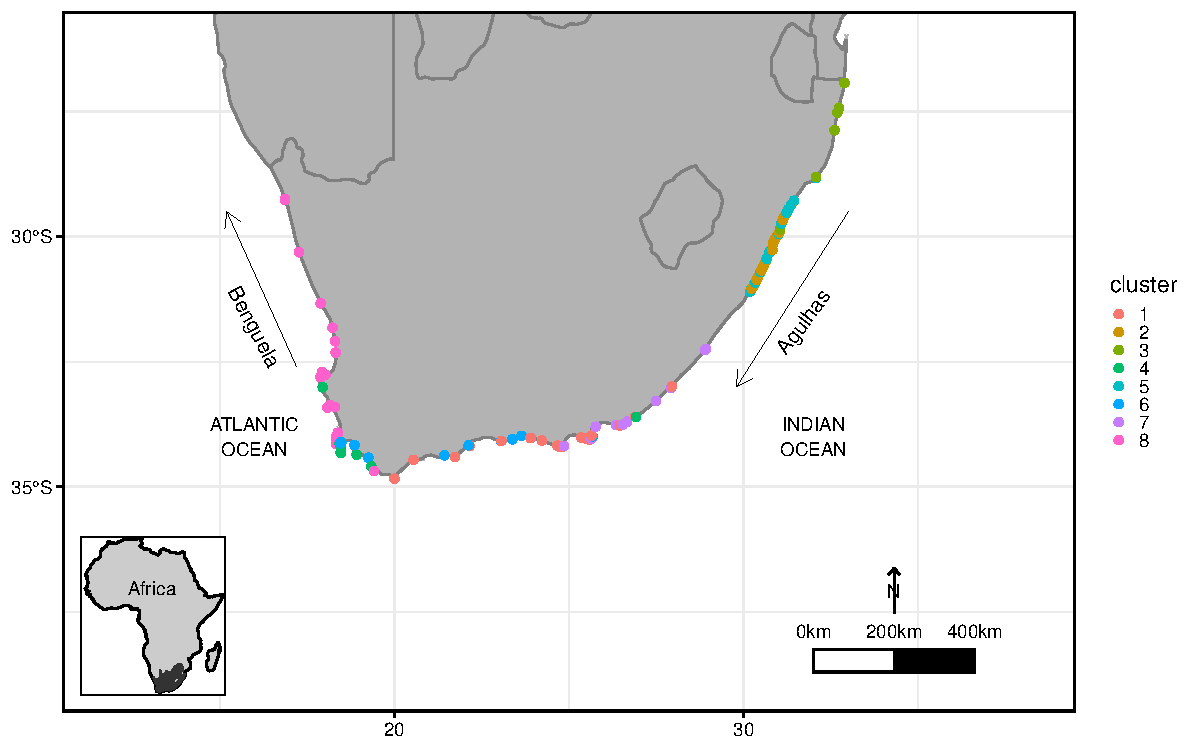
\includegraphics{figures/map_fixed.pdf}
\caption{Figure 1: A map of the study area representing the 129 sites
where \emph{in situ} coastal seawater temperature was collected. These
sites were grouped based on similar mean, minimum and maximum
temperatures and as such each groups represents a unique colour
variation.}
\end{figure}

Once sites were grouped together, the next step was to reduce the number
of sites down to a manageable, but still representative, sub-sample of
the whole. This was done primarily for two reasons. The first, simply,
was to allow for the comparisons to be more readily interpretable by
humans. Secondly it was to allow for equal amount of sampling per coast.
The east coast has previously been more heavily sampled than the rest
and such an imbalance should be addressed. The criteria considered for
the sub-samples included selecting the longest time series within the
region and including data from as many different organizations as
possible. This process yielded three sites for each of the clusters
along the South African coastline (Figure 2). The statistical
characteristics of the temperature were used to guide analysis of the
time series to produce an accurate assessment of temperature variation
between sites that were grouped together.
TalarifyTalarifyTalarifyTalarify
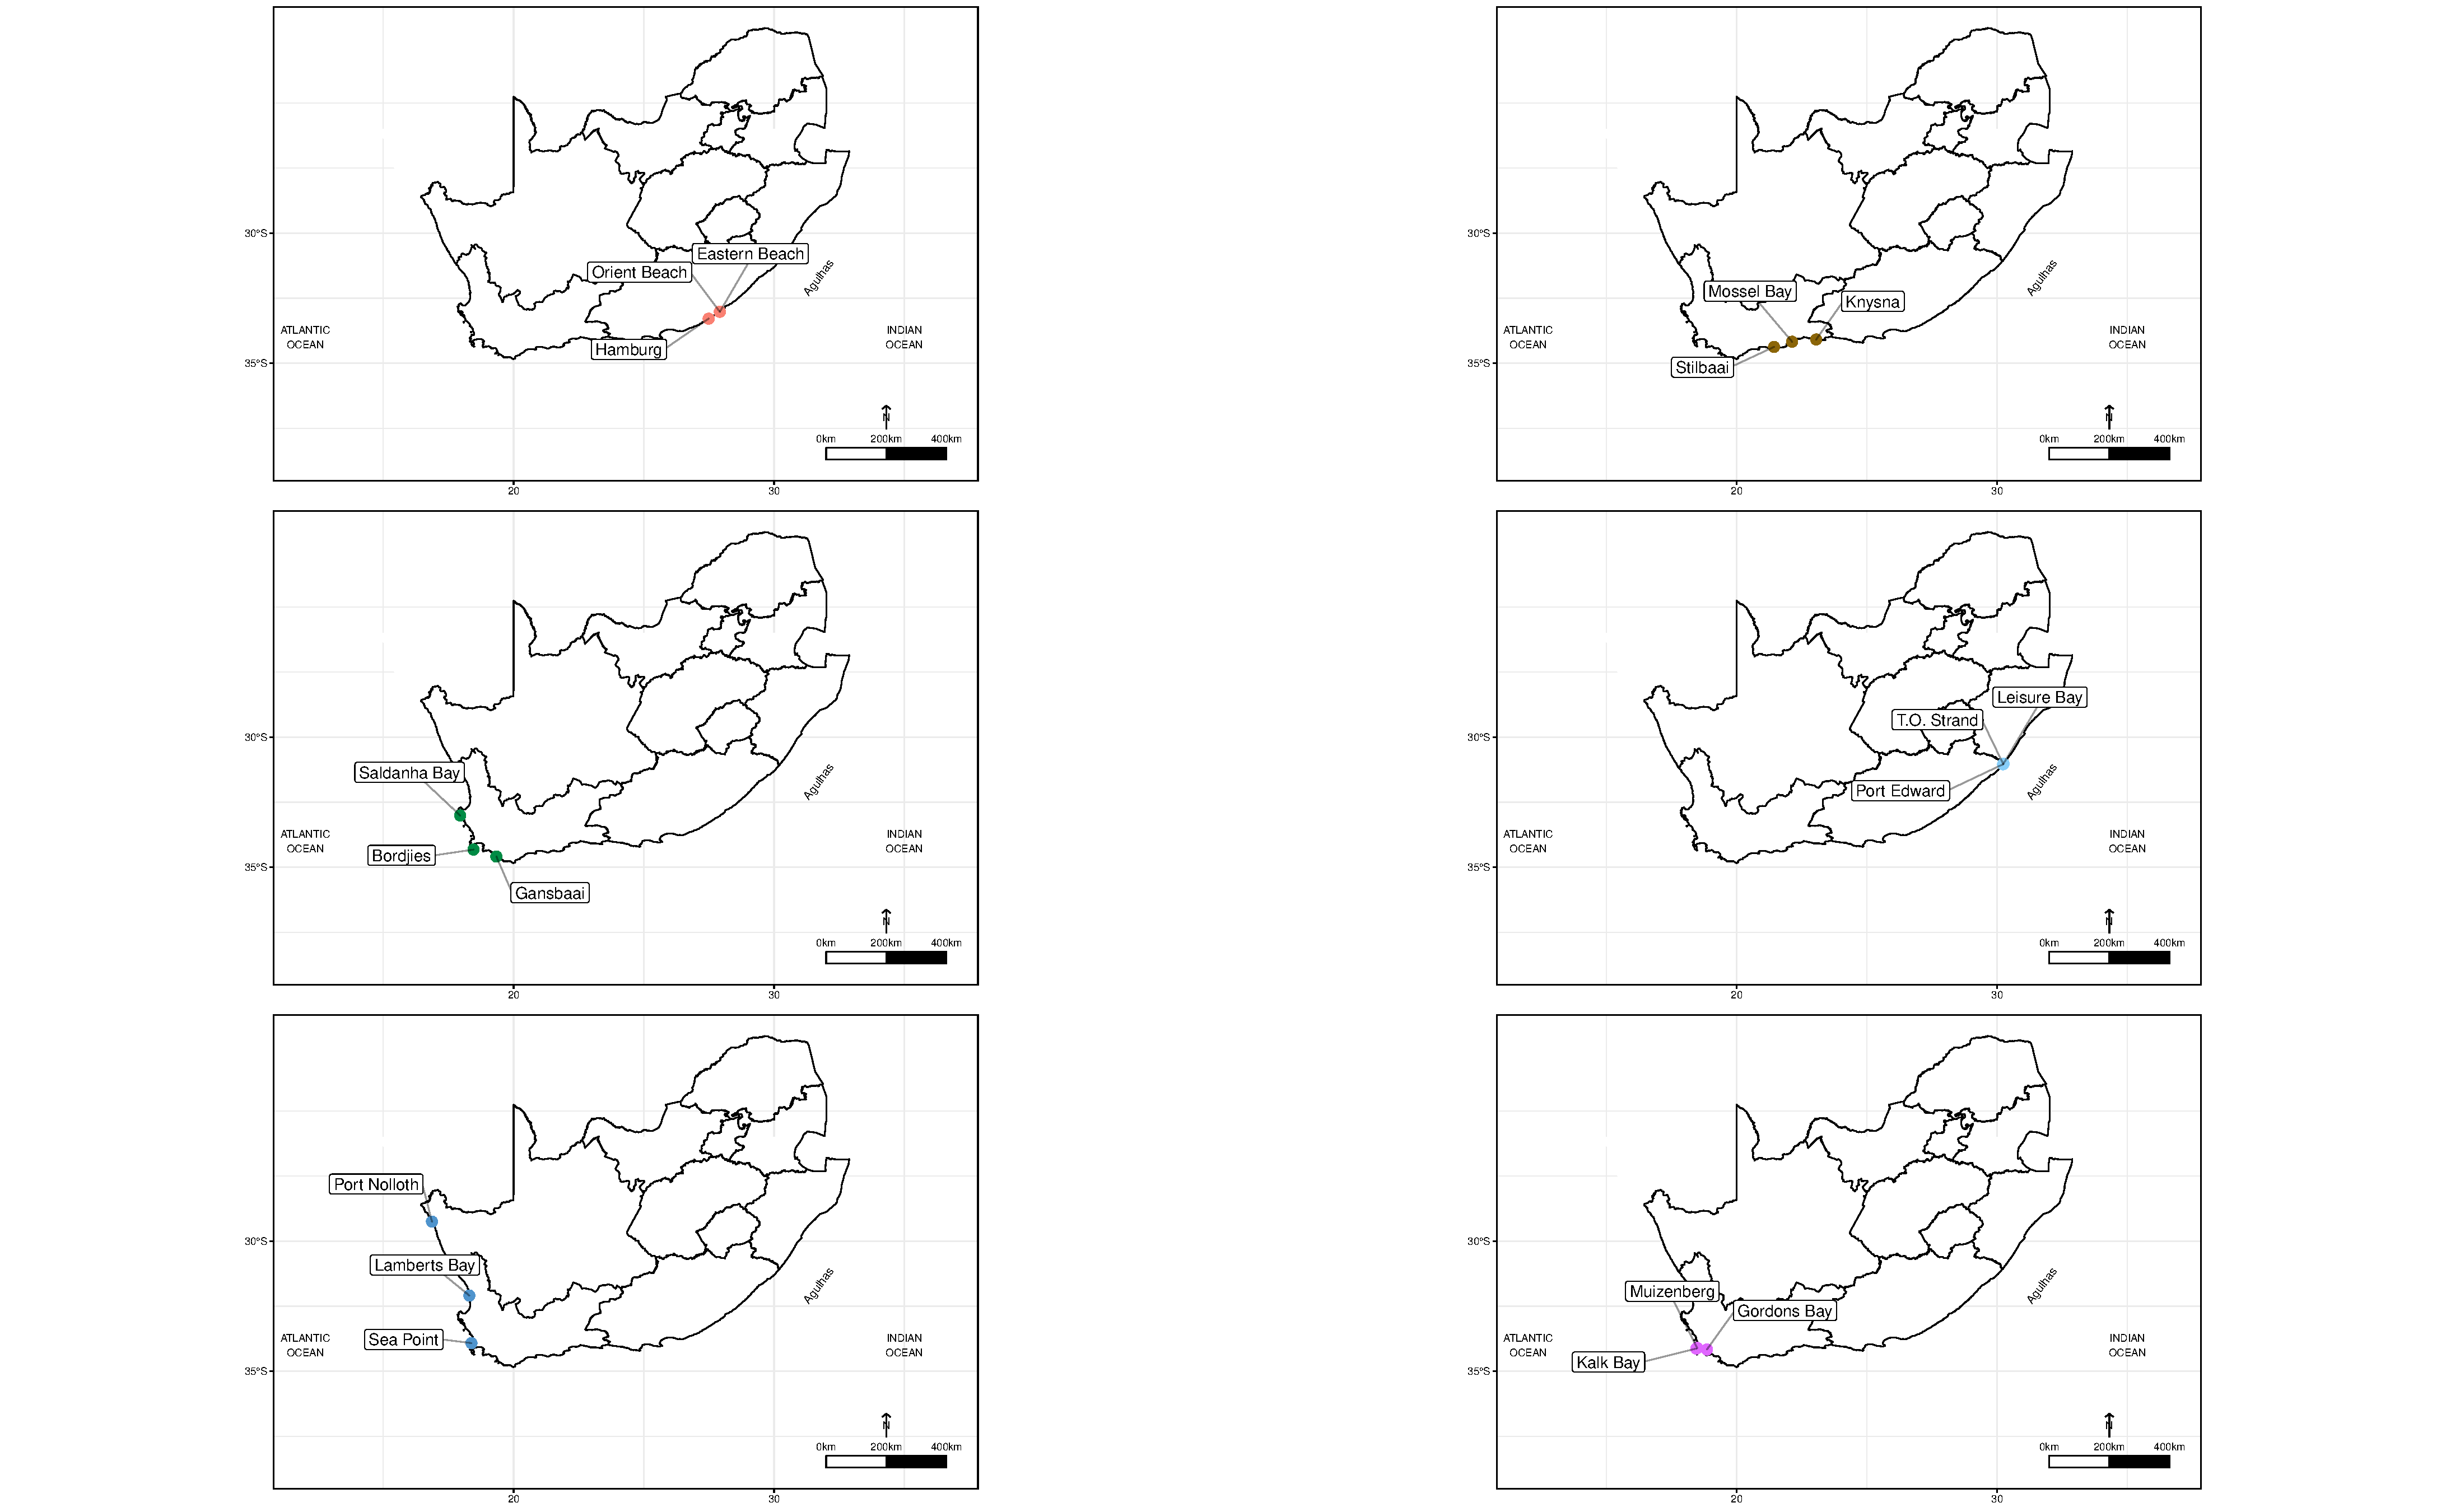
\includegraphics{figures/final_combined_plot.pdf}

With three sites per cluster, the haversine formula was used to
calculate the geodesic distance between points specified by radians.
Using this formula, the distances (km) between each of the sites along
the coastline were determined. Thereafter, sites within the same cluster
were matched based on the date that temperature was collected. This
allowed for a comparison to test whether or not temperature variation
exists between sites within the same cluster. Once the sites were
matched, the means and standard deviations of temperatures between sites
and clusters were determined. This highlighted the temperature variation
between matched sites and allowed for seasonal comparisons within the
same cluster.

Once the temperature variation between sites were carefully analysed,
the seawater temperature data along with the wave and wind data were
compared. Since the wave and wind data were collected at three hour
resolutions, they were converted into daily data points in order to
compare it with the temperature data. The wave data was collected at
depths of 7 m or 15 m respectively. The `circular' function in R
software was then used to create circular objects around the wave data
in order to calculate the daily wave and wind direction.

With temperature and wave values now corresponding to their respective
sites, depths and dates, the hypothesis regarding whether or not a
relationship existed between wind/wave action and temperature was
tested. To do this, linear models for each site was produced, reflecting
temperature and wave variations at each depth. Linear models typically
produce coefficients of determination R2 as an output, the `purrr'
function within the `tidyverse' R package was used to simultaneously
compare temperature and wave data across sites and depths. Hereafter,
ind and wave rose diagrams were constructed to determine the most
predominant direction for a particular site. This was done to ascertain
what the potential relationship between wind/waves and temperature was
at each site during only the prevailing wind/wave directions.

\subsection{Satellite data analysis}\label{satellite-data-analysis}

Sea Surface temperature measurements used in this study were obtained
from four different sources: MUR, CMC, K10 and AVHRR. A time series of
SST was determined by creating a bounding box which represented the
region of extent at the latitudes (-39.5° S, -25.5° S), and the
longitudes (10.5° E, 39.5° E). The size of the pixel search area was set
to use 2x the resolution of the sensor and at least 5x resol(km) from
each of the stations. The satellite datasets and the corresponding SACTN
\emph{in situ} collected dataset were matched based on the latitudes,
longitudes and the date at which temperature was collected. Some sites
however, shared the same satellite data due to their close proximities.
Once the satellite data corresponded with the \emph{in situ} collected
data, linear models for each site were produced, reflecting temperature
and wave variations at each depth. Linear models typically produce
coefficients of determination (R2 values) as an output, which is the
statistic showing how much of the variance in a dependent variable is
explained by the independent variable. This allows for us to test
whether or not wave and wind direction may influence temperature at the
various sites.

\subsection{Statistical analyses}\label{statistical-analyses}

A series of ANOVA tests were used to compare the main effects of the
chosen variables on a continuous variable. In this analysis the
relationship between matched sites based on the year and season as a
function of the mean temperature were analysed, these analyses were used
to test if significant differences occured between each pair of sites
within each of the clusters. To compare whether temperature variation
exist between sites found within the same clusters along the coast,
boxplots were constructed. These plots enabled the visual identification
of variations in temperature by summarising the descriptice statistics.
To furthur analyse the temperature variation between sites line graphs
were constucted. This plot allowed for visual identification of the
variation in average temperature for each of the month and year for
paired sites. All exploratory and statistical analyses were performed in
RStudio version 1.1.442 (\url{http://www.rstudio.com/}). The data used
within this study and comprehensive script used for data analyses, and
production of figures are to be found at
\url{https://github.com/AmierohAbrahams/HONOURSPROJECT}.

\subsection{Results}\label{results}

\subsubsection{Temperature variation}\label{temperature-variation}

Temperatures were not uniformly distributed across the six clusters
produced (Figure 3), with each set of sites having unique patterns of
temperature variation. In cluster 1, which included Humburg, Eastern
Beach and Orient Beach, it was found that temperature varied from
approximately 13 ºC to 22 ºC. Within this cluster of sites, Hamburg had
the highest maximum temperatures and the lowest minimum temperatures of
the three sites. Conversely, Orient Beach had the lowest range of
temperature variability, producing a comparatively short box plot.
Orient Beach and Eastern Beach had relatively similar ranges and
distributions of temperatures, as evident by their box plots nearly
overlapping completely.

Within the cluster comprised of Mossel Bay, Stilbaai, and Knysna,
temperatures ranged from approximately 12 ºC to 27 ºC, with most box
plots being relatively long. Stilbaai had the widest range of
temperature variation among the three sites but despite the apparent
differences in temperature ranges between these sites, the average
temperatures were relatively similar. Average temperatures were nearly
completely identical within this cluster, with very few outliers present
within the temperatures ranges of these sites.

Sites located within the third cluster had slightly lower temperatures
than the previous two clusters. This cluster comprised of Bordjies,
Saldanha, and Gansbaai and temperatures within here ranged from
approximately 11 ºC to 21 ºC, with an average median temperature being
close to 15 ºC across all three sites. Gansbaai had relatively low
variation in temperature as it had a comparatively short box plot.
Conversely, Saldanha had a long box plot representing high variation and
relatively evenly distributed temperatures. These sites were similar in
terms of their temperature variances, as their box plots were largely
overlapping with few differences between them. There were however
several outliers present within the temperatures of these sites.

The fourth cluster comprised of Port Edward, Leisure Bay, and T.O.
Strand. Overall, the temperatures of these sites were higher than those
of the sites within the other clusters, with a range of 15 ºC to 25 ºC,
which is considerably higher. The box plots for these sites were all
decidedly long, representing a low variation of temperature with little
skewness across sites. Temperatures did not differ between these three
sites with each box plot overlapping very well. The median temperature
for each of the sites within this cluster is 20.5 ºC.

Sites within the fifth cluster had overall lower temperatures than those
within the remaining clusters. This cluster comprised of Port Nolloth,
Lamberts Bay, and Sea Point, here sharp declines in average temperatures
were observed throughout. Temperatures within this cluster ranges
between 8 ºC and 18 ºC, with an average median temperature being close
to 13 ºC. Port Nolloth had low variation in temperature as it had a
comparatively short box plot with relatively evenly distributed
temperatures. Lamberts Bay and Sea Point were similar in terms of
temperature variances, as their box plots were largely overlapping with
little differences between them. Several outliers were present within
the temperatures of these sites.

In the cluster comprising of Kalk Bay, Muizenberg, and Gordons Bay the
temperatures of these sites ranged from 8 ºC to 24 ºC, with most box
plots being short. Muizenberg had the widest range of temperature
variation of the three sites. Gordons Bay and Kalk Bay had identical
temperature ranges. Similarly to the second cluster, despite the
apparent differences in temperature ranges between these sites, the
average temperatures across them were relatively similar and nearly
identical.

\begin{figure}
\centering
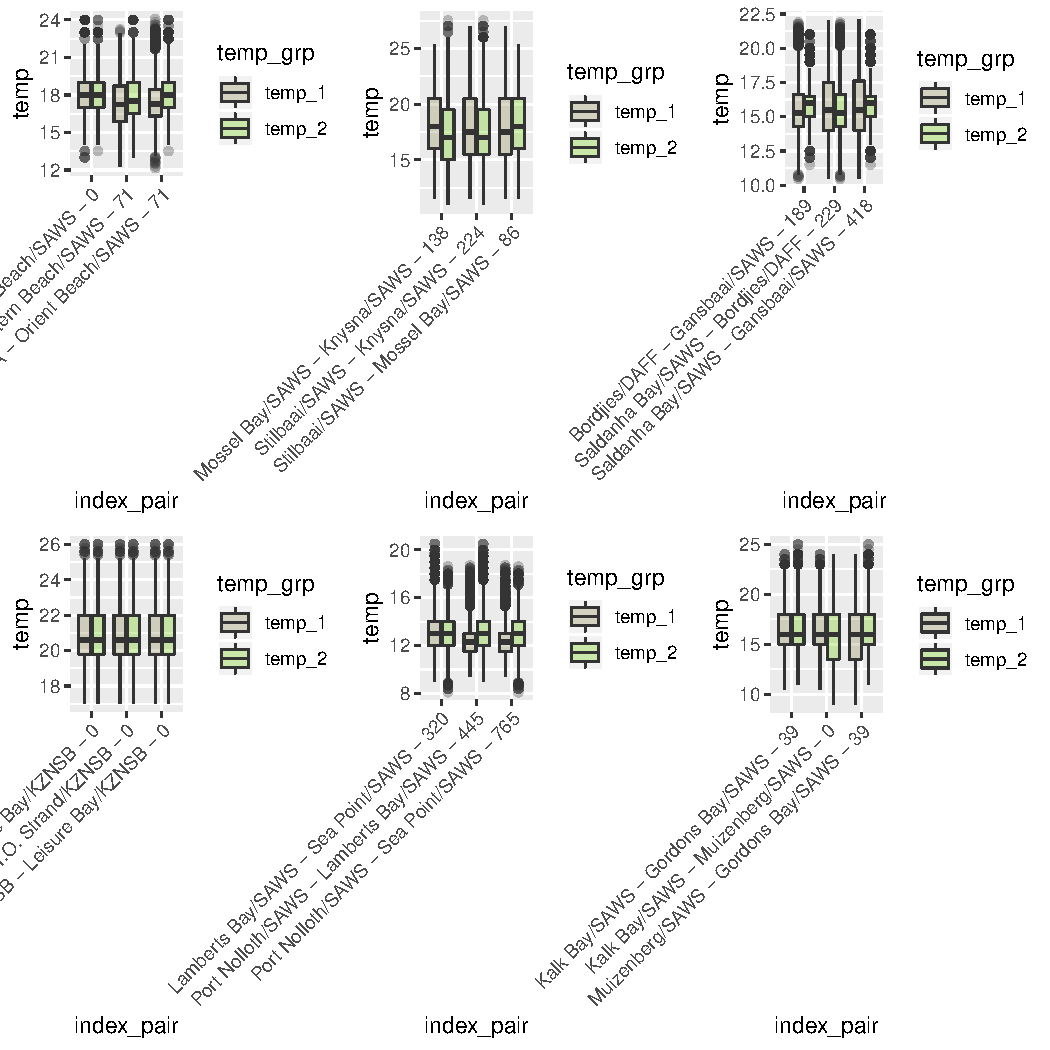
\includegraphics{figures/combined_plot.pdf}
\caption{Figure 3: Boxplots representing the difference in seawater
temperature of paired sites within each cluster along the South African
coast.}
\end{figure}

On a monthly basis, the differences of average temperatures between
sites within cluster 1, Eastern Beach, Orient Beach and Humburg,a large
average temperature variation between Hamburg and Eastern Beach were
seen during the summer and spring months of 1995 to 1997. For the
remaining sites however, differences in average temperatures were low
during Autumn. It was also evident that the average temperature between
Hamburg and Orient Beach varied largely on an apparent seasonal basis.
Slight average temperature variation existed between Eastern Beach and
Orient Beach throughout the different seasons.

Converse to the first cluster, the cluster containing Mossel Bay, Knysna
and Stilbaai, the largest differences in average temperatures were
observed during autumn and winter months. In this cluster large
differences in average temperatures were present between Mossel Bay and
Knysna, with the differences increasing annually from 1985 to 2017.
Similarly, differences in average temperature also increased slightly
between Stilbaai and Knysna during winter and spring. During summer
months little differences in average temperature varation were seen
between all three sites within this cluster.

Differences of average temperatures between sites within cluster 3
(Bordjies, Gansbaai and Saldanha) varied on an apparent seasonal basis.
During the summer months we saw that there were large differences in
average temperatures between Bordjies and the remaining three sites,
with an increase in differences of average temperature between Saldanha
Bay and Gansbaai throughout autumn, winter and spring.

In the fourth cluster, which comprised of Port Edward, Leisure Bay and
T.O. Strand, small changes in the differences of average temperatures
were notticed between sites on a monthly basis between 1980 to 2017.
Here, the large differences in temperatures were observed towards the
end of spring and during summer months. Temperatures were relatively
stable throughout winter and the beginning of spring across all three
sites found within this cluster.

In the cluster containing Lamberts Bay, Port Nolloth and Sea Point,
large differences in average temperatures between sites at selected
months between 1972 and 2017. During summer and Autumn months,
differences in average temperature were observed between Lamberts Bay
and the remaining sites increased. During the months of autumn Lamberts
Bay and Seapoint showed large differences in average temperature
variation. For the remaining sites, differences in average temperatures
were relatively low throughout each month for the same time period.

In the cluster comprising of Kalk Bay, Gordons Bay and Muizenberg, the
largest differences in average temperatures were observed during mid
autumn and winter months. In this cluster large differences in average
temperatures were seen between Muizenberg and the remaining sites, with
the differences increasing annually throughout 1972 and 2016 during
winter. Similarly, differences of average temperatures also increased
between Kalk Bay and Muizenberg during these same months. In the summer
and spring months little differences in average temperatures between
sites, with minimal differences in the rates of these changes. These
rates increased during spring.

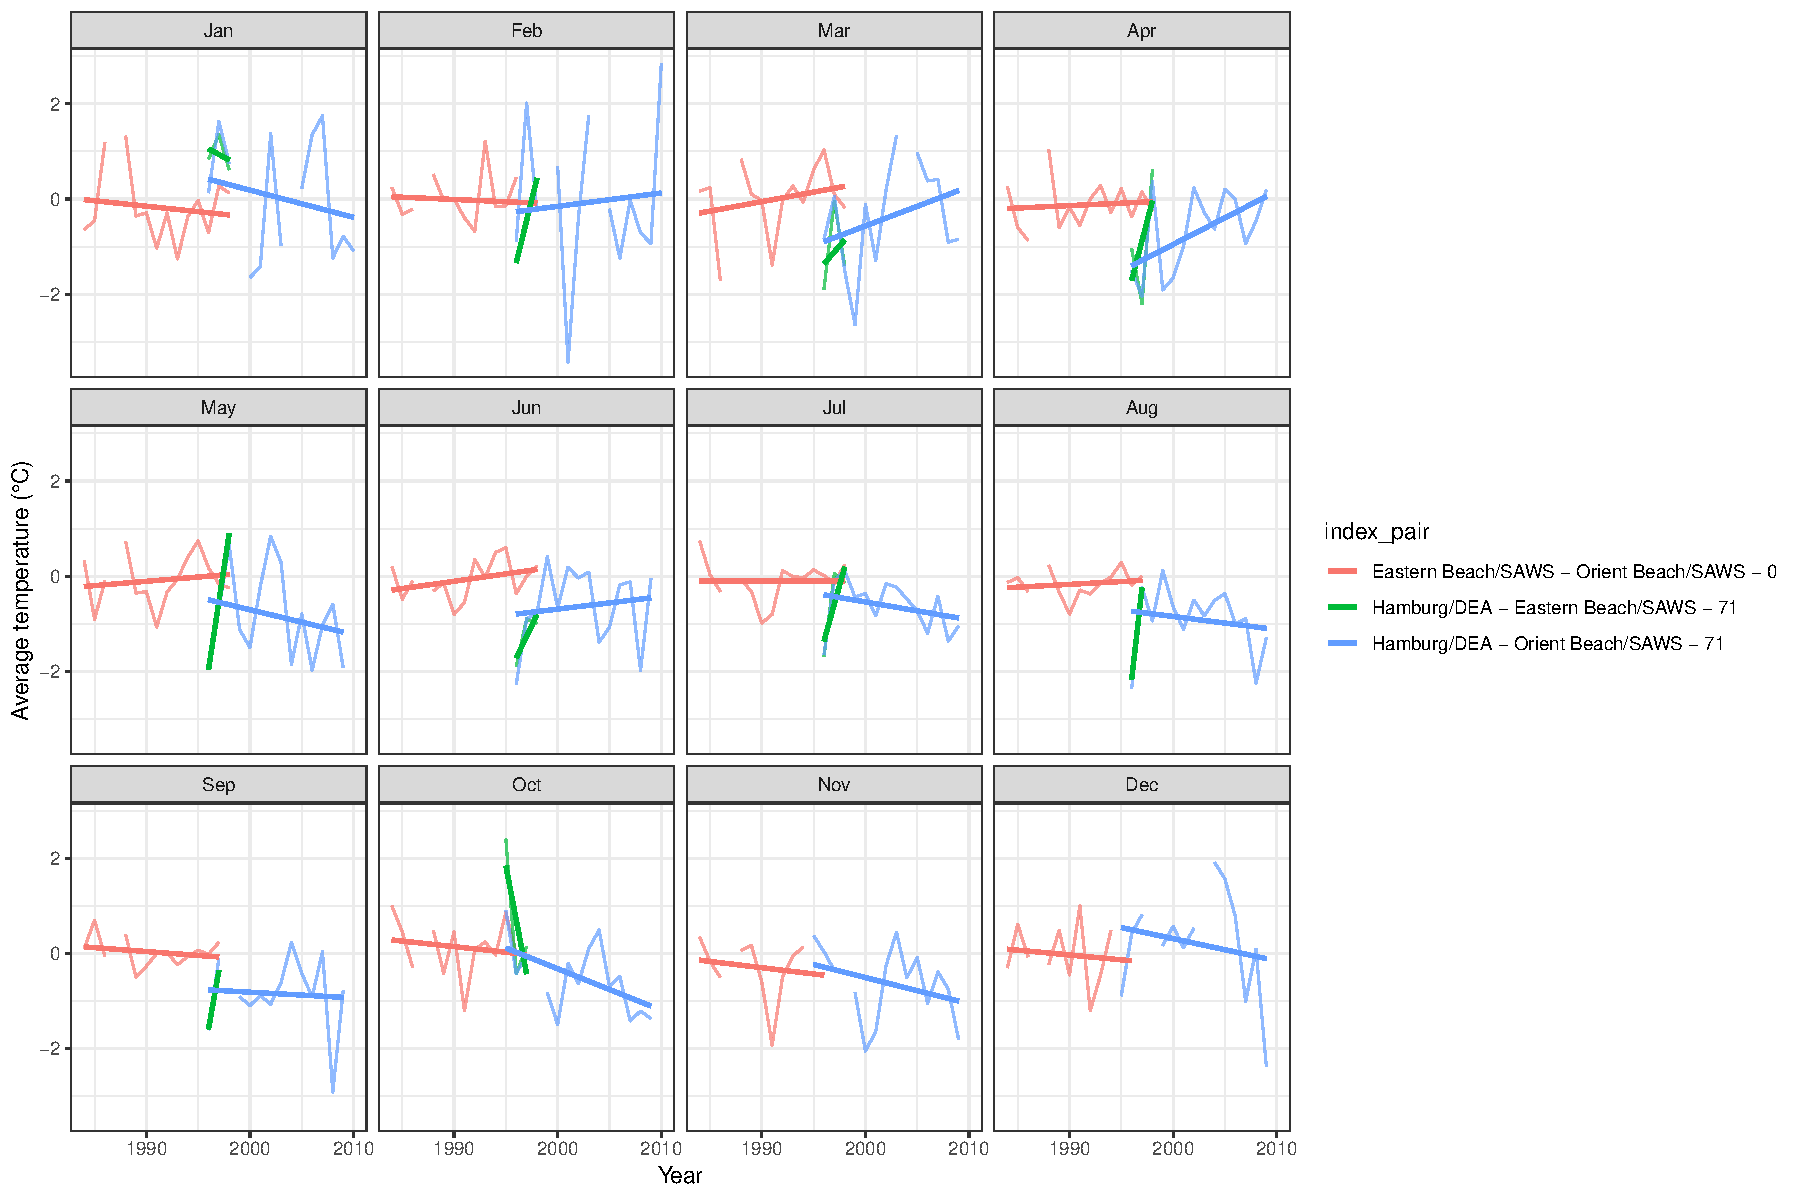
\includegraphics{figures/SACTN_clust_1_plot2.pdf}
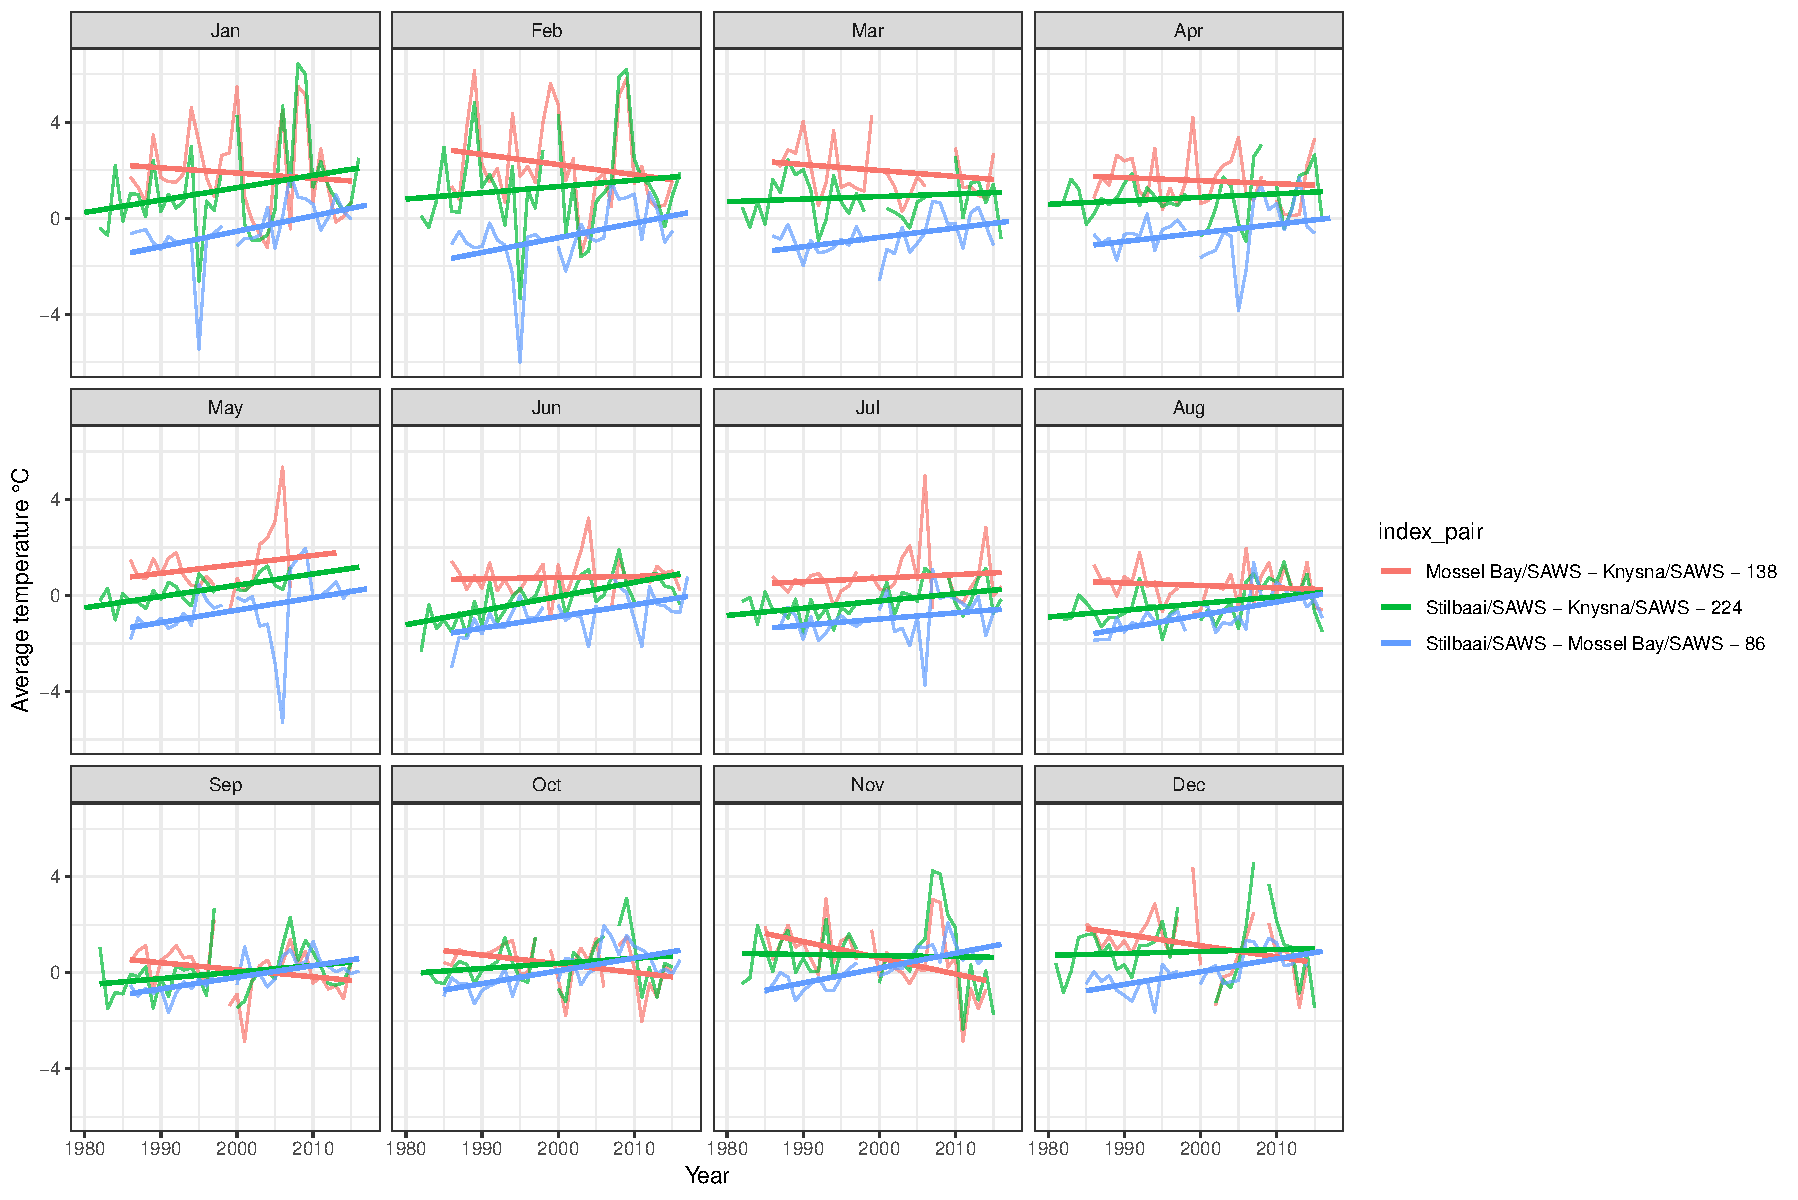
\includegraphics{figures/SACTN_clust_2_plot2.pdf}
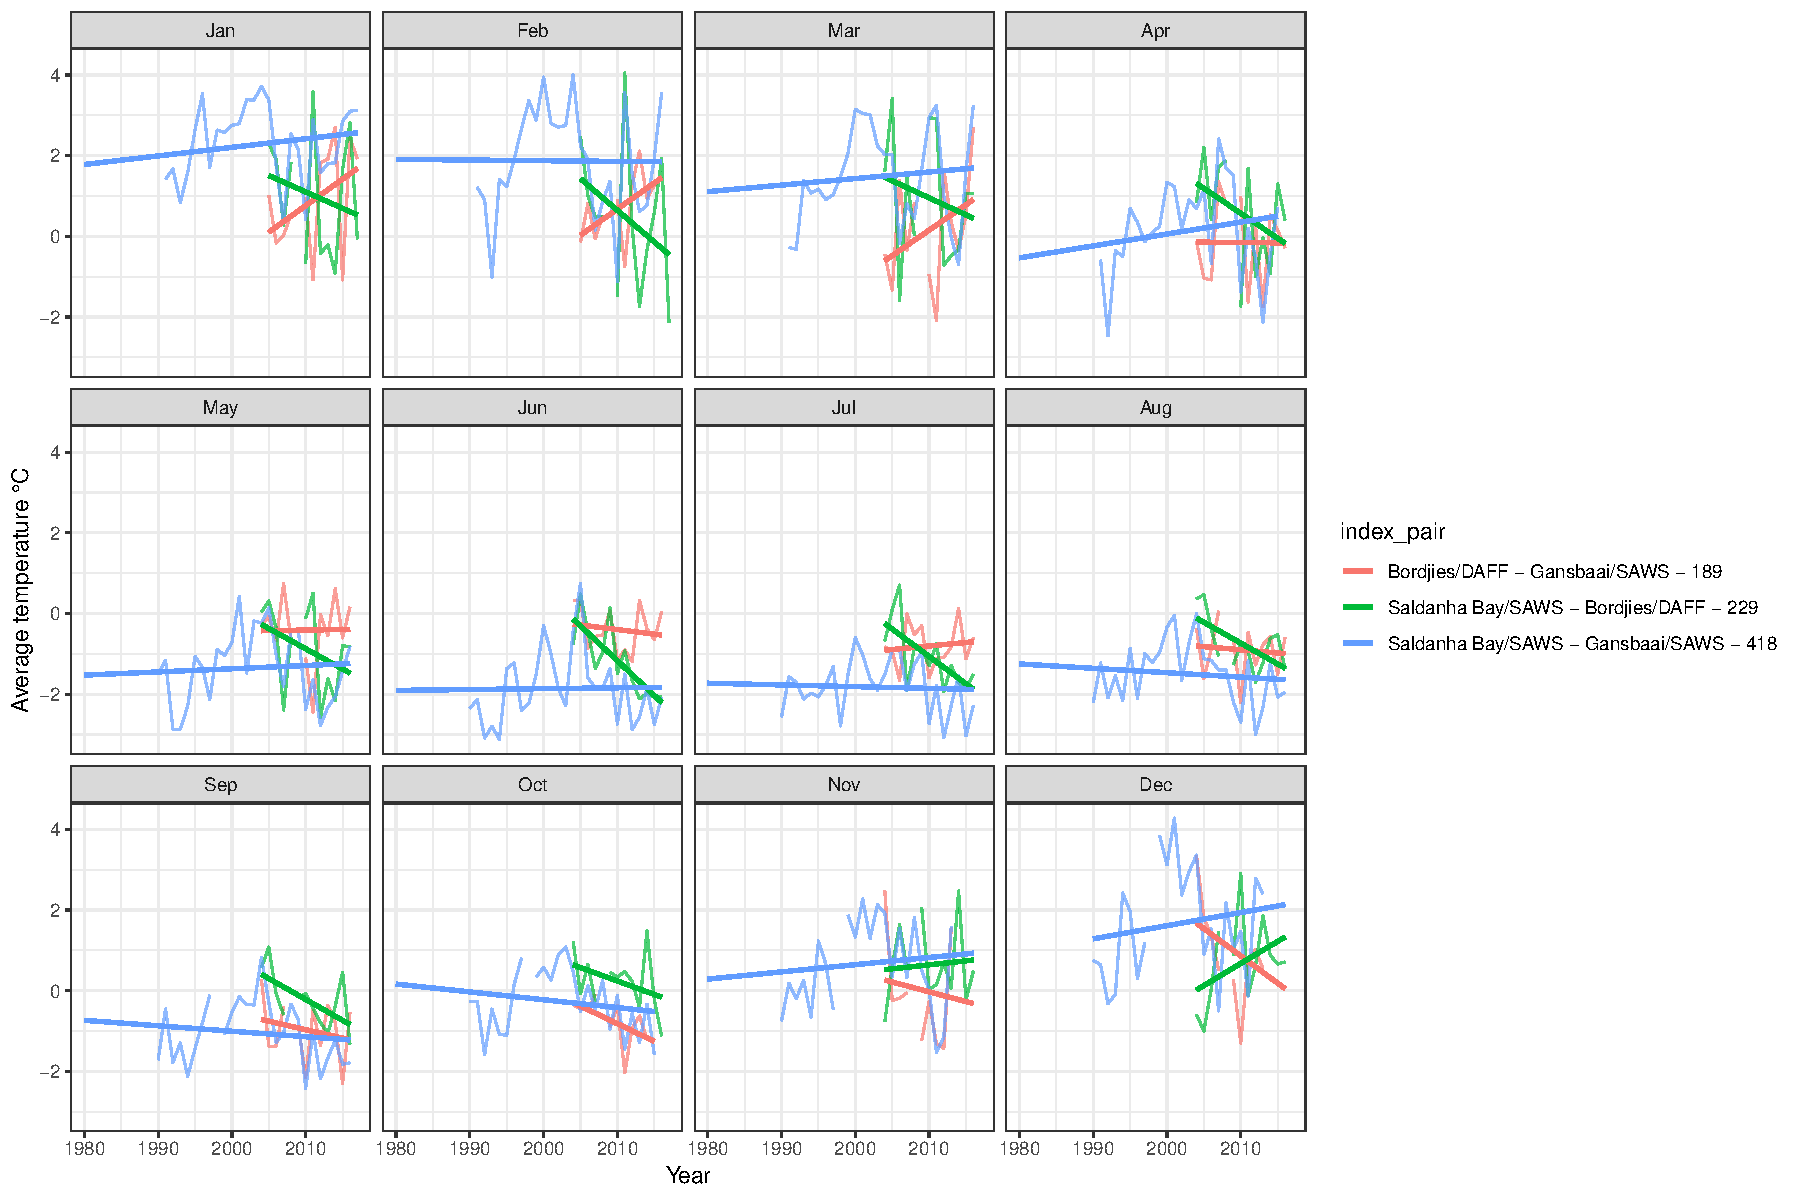
\includegraphics{figures/SACTN_clust_3_plot2.pdf}
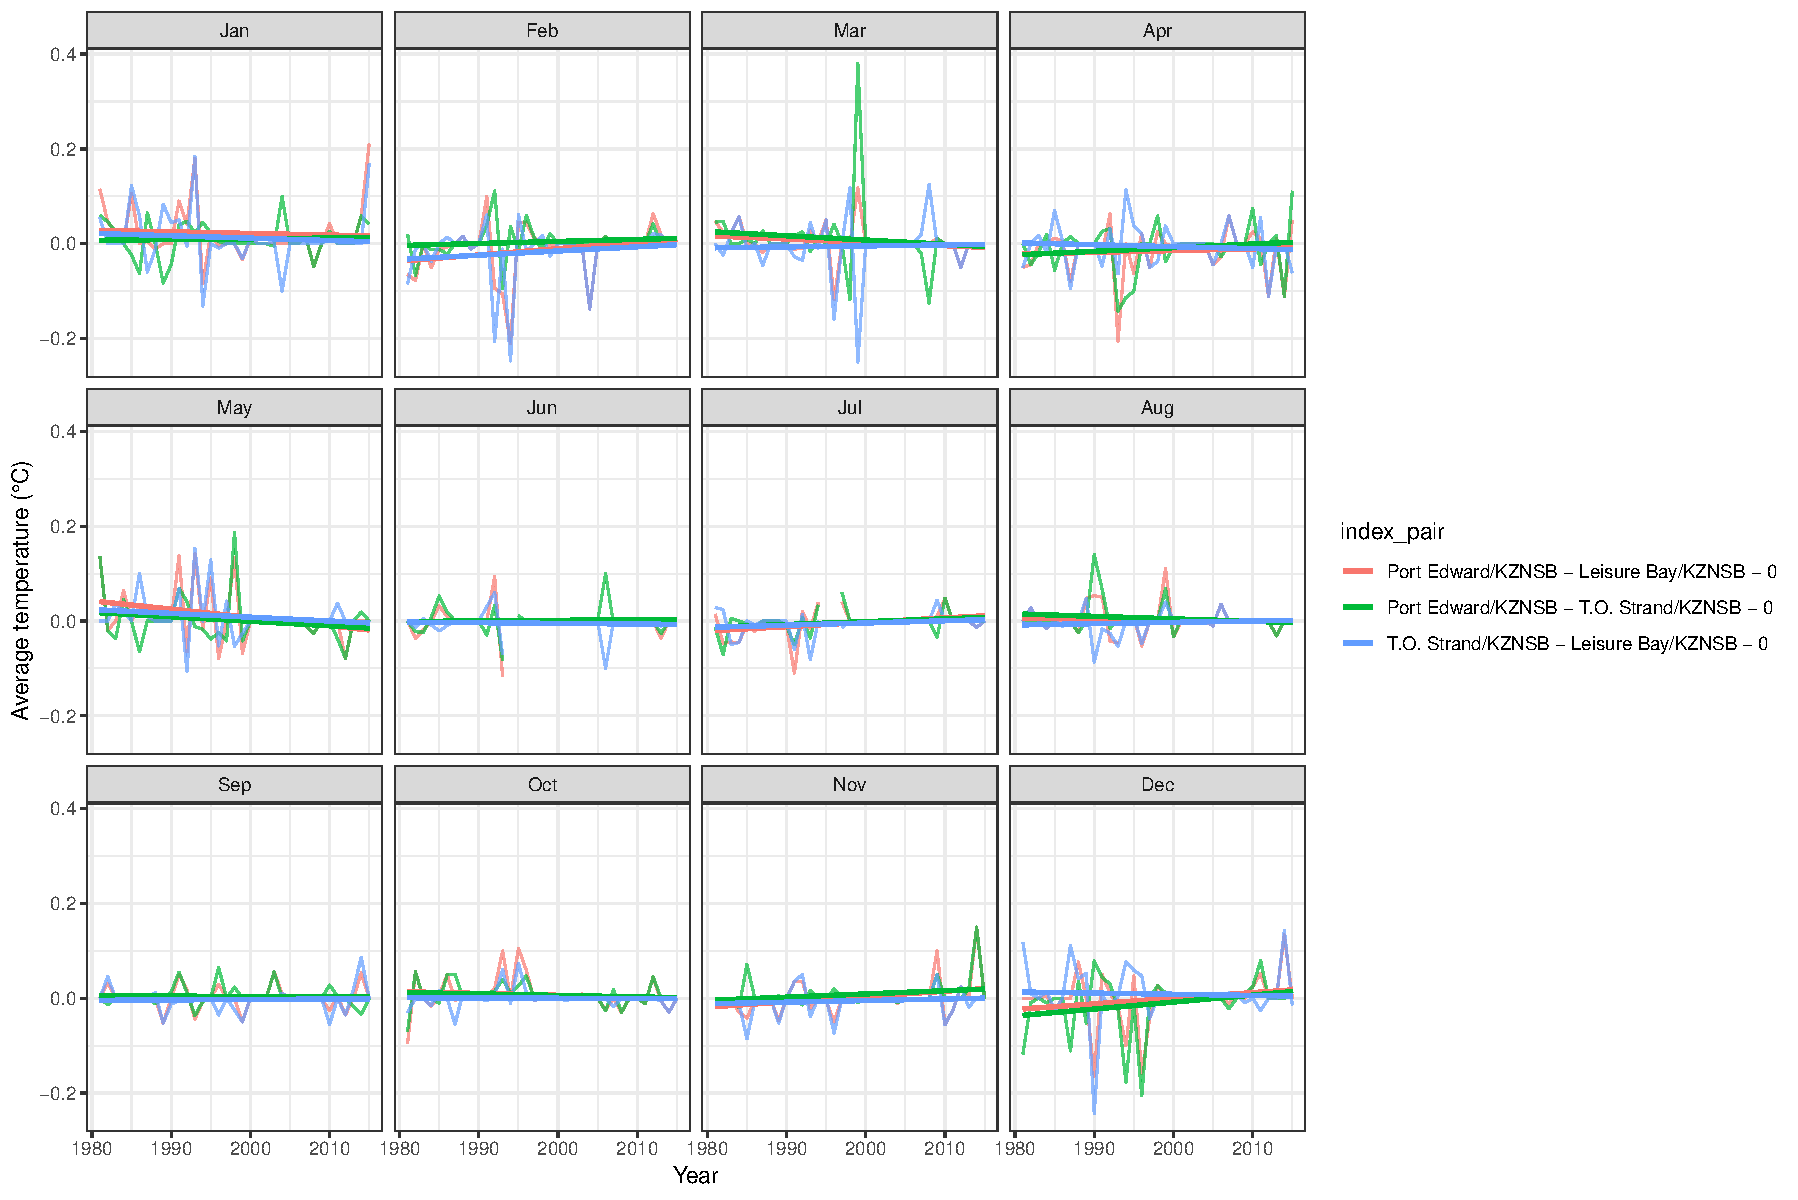
\includegraphics{figures/SACTN_clust_4_plot2.pdf}
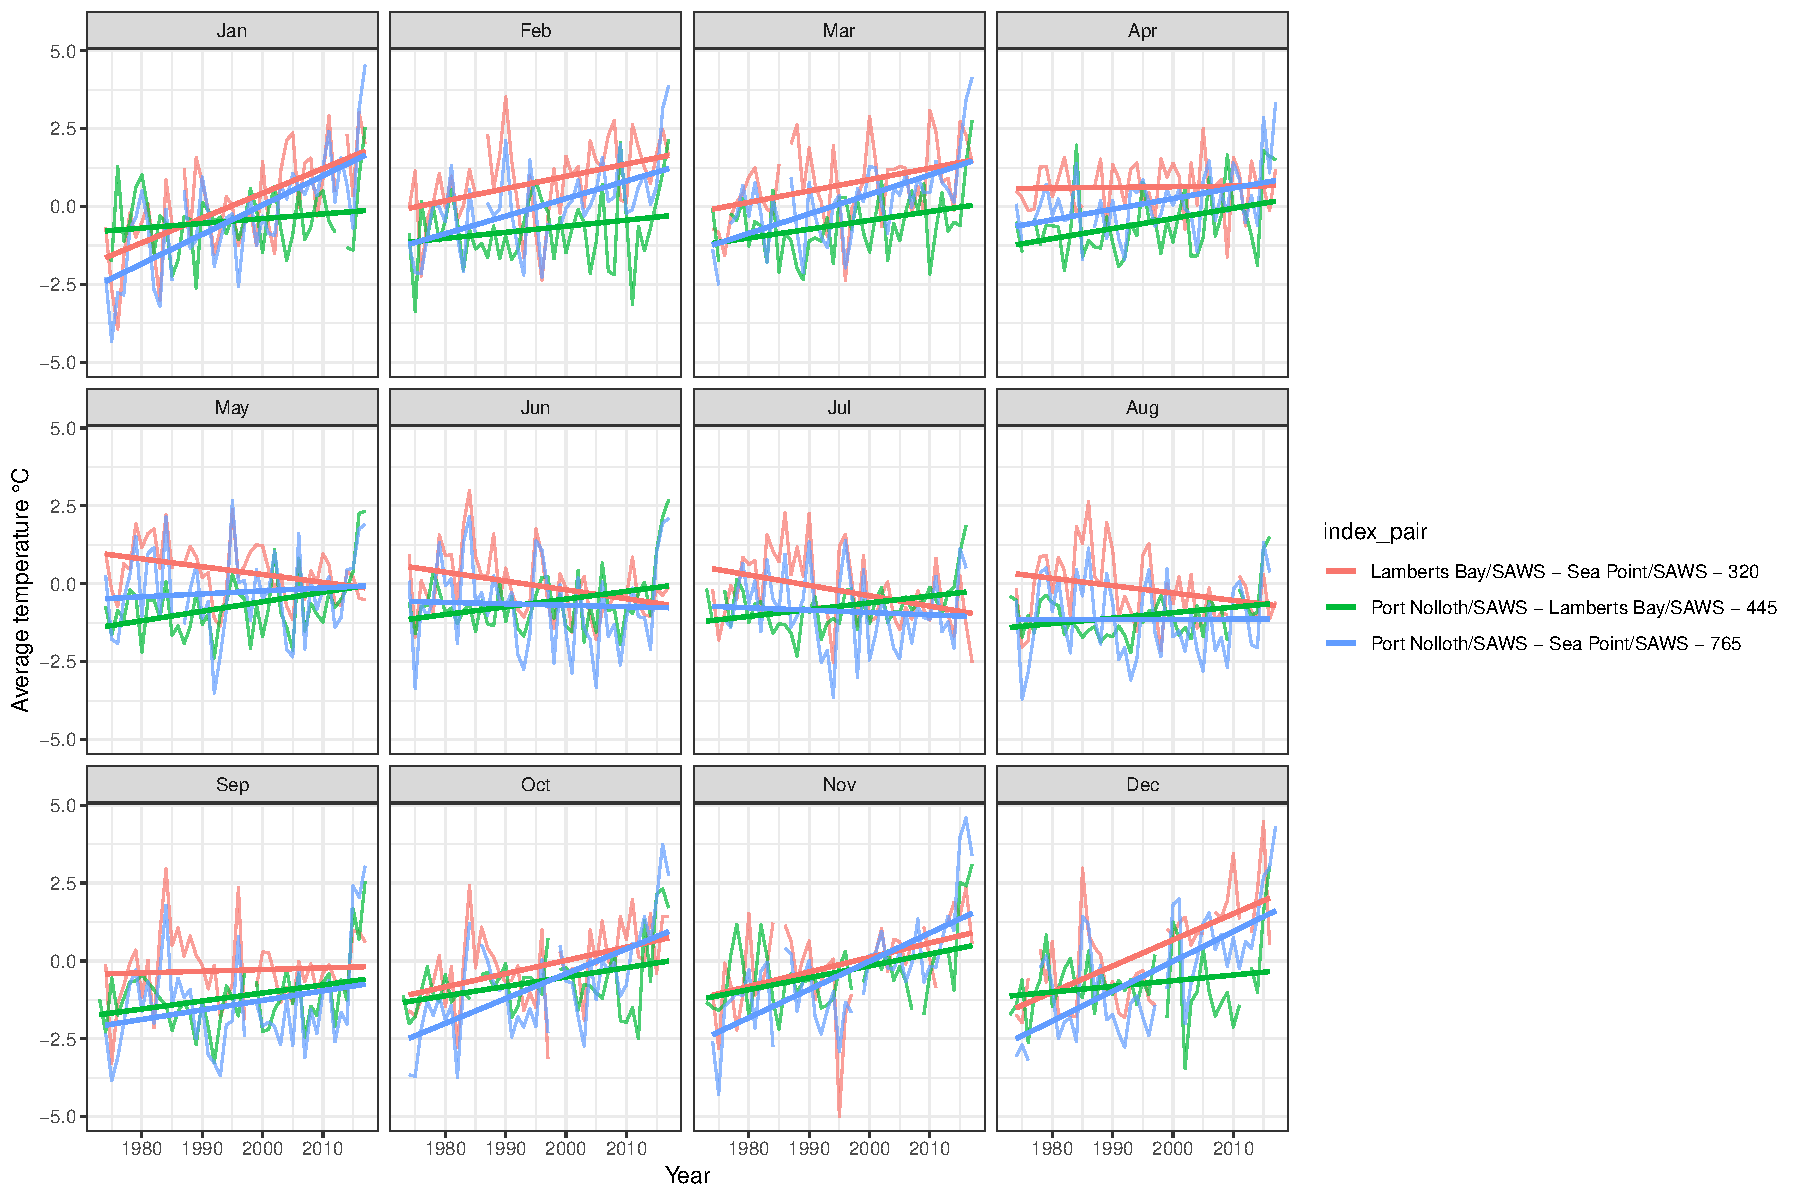
\includegraphics{figures/SACTN_clust_5_plot2.pdf}
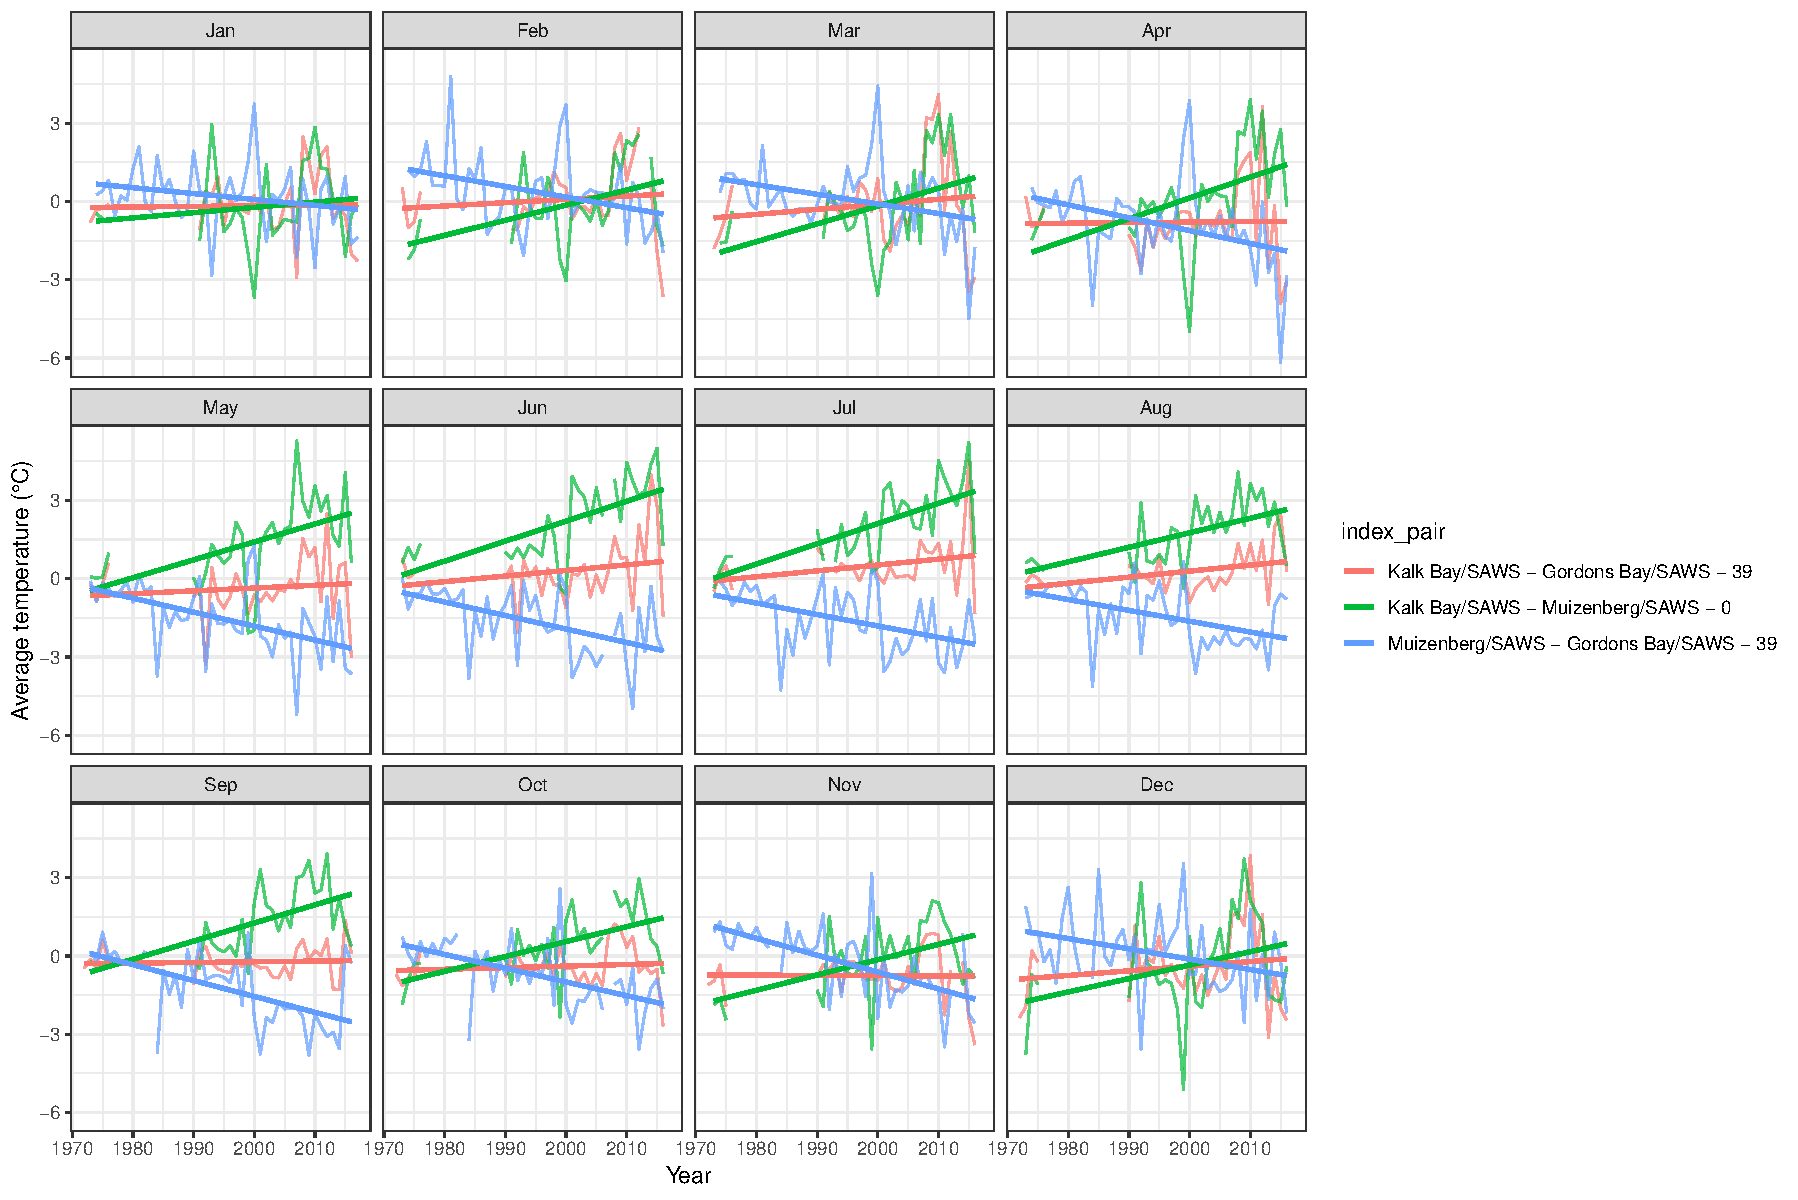
\includegraphics{figures/SACTN_clust_6_plot2.pdf}

\subsubsection{Average temperature of clustered
sites}\label{average-temperature-of-clustered-sites}

In the first cluster of sites, via the results of a one way ANOVA tests
it was found that there was a significant differences in average
temperatures between paired sites (F2 = 12.07, SS = 15.28, P \textless{}
0.001). These differences were present across season (F6 = 3.44, SS =
13.07, P \textless{} 0.002) but were not present yearly between
individuals and paired sites (F2 = 1.38, SS = 1.75, P = 0.25).
Similarly, paired sites within the second cluster also a significantly
differed in average temperature (F2 = 166.84, SS = 418.6, P \textless{}
0.001). Conversely to first cluster however these differences were
present yearly (F1 = 33.21, SS = 41.7, P \textless{} 0.001) and
seasonally (F6 = 16.72, SS = 125.9, P \textless{} 0.02,) between
individual and paired sites. In the third cluster of sites, ANOVA tests
revealed that there were no significant differences in average
temperatures between paired sites (F2 = 1.17, SS = 2.9, P = 0.31), but
temperatures varied seasonally and yearly between individual sites (. In
the fourth cluster there were again no significant difference of average
temperatures between paired sites (F2 = 0.73, SS = 2.9, P = 0.48).
Differences were also absent across seasons (F3 = 0.75, SS = 0.0042, P =
0.52) and years (F1 = 0.495, SS = 0.0009, P = 0.48) between both
individual and paired sites. Sites within the fifth cluster were
significantly different in average temperatures between paired sites (F2
= 77.10, SS = 196.7, P \textless{} 0.002), with these differences being
present yearly (F1 = 172.80, SS = 220.4, P \textless{} 0.001) and
seasonally (F3 = 77.10, SS = 29.92, P \textless{} 0.002) for both paired
and individual sites. Finally, sites within the sixth cluster also
significantly difference in average temperatures between paired sites,
yearly and seasonally (F2 = 132.044, SS = 419.7, P \textless{}0.01).

\subsection{The coefficient of
determination}\label{the-coefficient-of-determination}

\begin{longtable}[]{@{}l@{}}
\caption{A table showing the impact of wind and wave action at a depth
of 7 meters for the SACTN temperature dataset}\tabularnewline
\toprule
x\tabularnewline
\midrule
\endfirsthead
\toprule
x\tabularnewline
\midrule
\endhead
SACTN\_15\_R2\tabularnewline
\bottomrule
\end{longtable}

\begin{longtable}[]{@{}l@{}}
\caption{A table showing the impact of wind and wave action at a depth
of 15 meters for the SACTN temperature dataset}\tabularnewline
\toprule
x\tabularnewline
\midrule
\endfirsthead
\toprule
x\tabularnewline
\midrule
\endhead
SACTN\_15\_R2\tabularnewline
\bottomrule
\end{longtable}

\begin{longtable}[]{@{}l@{}}
\caption{A table showing the impact of wind and wave action at a depth
of 7 meters for the AVHRR temperature dataset}\tabularnewline
\toprule
x\tabularnewline
\midrule
\endfirsthead
\toprule
x\tabularnewline
\midrule
\endhead
AVHRR\_temp\_7\_R2\tabularnewline
\bottomrule
\end{longtable}

\begin{longtable}[]{@{}l@{}}
\caption{A table showing the impact of wind and wave action at a depth
of 15 meters for the AVHRR temperature dataset}\tabularnewline
\toprule
x\tabularnewline
\midrule
\endfirsthead
\toprule
x\tabularnewline
\midrule
\endhead
AVHRR\_temp\_15\_R2\tabularnewline
\bottomrule
\end{longtable}

\begin{longtable}[]{@{}l@{}}
\caption{A table showing the impact of wind and wave action at a depth
of 7 meters for the MUR temperature dataset}\tabularnewline
\toprule
x\tabularnewline
\midrule
\endfirsthead
\toprule
x\tabularnewline
\midrule
\endhead
MUR\_7\_R2\tabularnewline
\bottomrule
\end{longtable}

\begin{longtable}[]{@{}l@{}}
\caption{A table showing the impact of wind and wave action at a depth
of 15 meters for the MUR temperature dataset}\tabularnewline
\toprule
x\tabularnewline
\midrule
\endfirsthead
\toprule
x\tabularnewline
\midrule
\endhead
MUR\_15\_R2\tabularnewline
\bottomrule
\end{longtable}

\begin{longtable}[]{@{}l@{}}
\caption{A table showing the impact of wind and wave action at a depth
of 7 meters for the CMC temperature dataset}\tabularnewline
\toprule
x\tabularnewline
\midrule
\endfirsthead
\toprule
x\tabularnewline
\midrule
\endhead
CMC\_7\_R2\tabularnewline
\bottomrule
\end{longtable}

\begin{longtable}[]{@{}l@{}}
\caption{A table showing the impact of wind and wave action at a depth
of 15 meters for the CMC temperature dataset}\tabularnewline
\toprule
x\tabularnewline
\midrule
\endfirsthead
\toprule
x\tabularnewline
\midrule
\endhead
CMC\_15\_R2\tabularnewline
\bottomrule
\end{longtable}

\begin{longtable}[]{@{}l@{}}
\caption{A table showing the impact of wind and wave action at a depth
of 7 meters for the K10 temperature dataset}\tabularnewline
\toprule
x\tabularnewline
\midrule
\endfirsthead
\toprule
x\tabularnewline
\midrule
\endhead
K10\_7\_R2\tabularnewline
\bottomrule
\end{longtable}

\begin{longtable}[]{@{}l@{}}
\caption{A table showing the impact of wind and wave action at a depth
of 15 meters for the K10 temperature dataset}\tabularnewline
\toprule
x\tabularnewline
\midrule
\endfirsthead
\toprule
x\tabularnewline
\midrule
\endhead
K10\_15\_R2\tabularnewline
\bottomrule
\end{longtable}

\section{The impact of wind and wave action on temperature at a depth of
7meters}\label{the-impact-of-wind-and-wave-action-on-temperature-at-a-depth-of-7meters}

\subsection{SACTN:}\label{sactn}

The coeffcient of determination was calculated to determine the
relationship between temperature and several variables including wind
direction and speed as well as wave height, period, direction and speed,
for all 18 sites. The results showed little variation in environmental
factors and temperature for each of the sites. Wind and wave direction
influenced temperature at 0 -- 3\%. The most significant relationships
were found in Muizenberg, Kalk Bay and Mossel Bay where the R\^{}2
values indicated that wave period had a 6-7\% influence on temperature.

\subsection{AVHRR:}\label{avhrr}

Upon examining the impact of wind and wave action on seawater
temperature, it was seen that wave and wind direction had a minimal
effect on temperature variation with its R\^{}2 values ranging between
0-3\%. The results also indicated that wave height influenced
temperature at some of the sites. This was evident in Gaansbaai and
Lamberts Bay where wave height had a 9\% impact on temperature
variation.

\subsection{MUR:}\label{mur}

The results continued to show little variation in regards to the
influence of wind and wave action on temperature. At many of the sites,
both wind and wave direction had a 0\% impact on the temperature.
However, it was seen that wave height and wave period had the greatest
impact on temperature at some of the sites, with Gordons Bay and
Gaansbaai indicating an 8\% and 10\% impact of wave height on
temperature variation respectively.

\subsection{CMC:}\label{cmc}

The results indicated that wave as well as wind direction and wind speed
showed the least significant impact on temperature variation with r\^{}2
values ranging between 0-3\%. Wave height continued to show the largest
impact on temperature variation at some of the sites. Here, Gaansbaai
and Gordons Bay indicated the highest R\^{}2 values of 12\% and 9\%
respectively.

\subsection{K10:}\label{k10}

When comparing the impact of various environmental factors on
temperature variation for the K10 data, the results indicated that the
each of the above-mentioned variables had no impact on the temperature
variation at Hamburg. The impact of wind direction on temperature is
highest at Gansbaai, representing an R\^{}2 value of 4\%. Wave height
still repersented the greatest influence on temperature occurring at
these sites

\section{The impact of wind and wave action on temperature at a depth of
15meters}\label{the-impact-of-wind-and-wave-action-on-temperature-at-a-depth-of-15meters}

\subsection{SACTN:}\label{sactn-1}

The coefficient of determination was calculated to determine the
relationship between temperature and several variables including wind
direction and speed as well as wave height, period, direction and speed,
for all 18 sites. The analyses indicated that there was no relationship
present between the above-mentioned factors at Eastern Beach. Wave
direction was seen to have no influence on temperature at any of the
sites analysed as the R\^{}2 values were at a constant 0\%. Wind
direction exhibited relationships between 0-4\% across all sites,
indicating that that factor did not significantly influence coastal
temperature. The most significant relationships were found at the
Muizenberg and Kalk Bay sites where the R\^{}2 values indicated that
wave period had an 8\% and 7\% influence on temperature respectively.

\subsection{AVHRR:}\label{avhrr-1}

The analyses indicated that a relationship existed between each of the
environmental variables at Stilbaai with the intensity of these
variables on temperature being extremely low. Wave period and wave
height at Port Nolloth and Lamberts Bay represented the largest
influence on temperature variation. This was still low with R\^{}2
values between 6\% - 8\%. In Gaansbaai wave height had a 9\% influence
on temperature, this being the largest value recorded.

\subsection{MUR:}\label{mur-1}

Upon examining the relationship between the MUR SST dataset and each of
the environmental factors it was found that wave height and wave period
of each of the sites had the greatest influence on temperature variation
compared to any of the other variables. Similarly to the AVHRR dataset,
Gaansbaai is largely influenced by wave height as indicated by R\^{}2
value of 10\%. Stillbaai and Seapoint also indicated that wave height
had a 7\% and 6\% influence on temperature respectively. Muizenberg
however, was the only site present where wave height had a 0\% influence
on temperature.

\subsection{CMC:}\label{cmc-1}

In the CMC SST dataset it was seen that wave height was the main factor
influencing temperature at these sites. Gansbaai represented a R\^{}2
value of 12\% which was the highest value for each of the variables
within this dataset. Each of the other environmental variables appeared
to have a minor influence on the temperature for each of the sites
ranging between 0\% - 4\%

\subsection{K10:}\label{k10-1}

When comparing the relationship between SST of the K10 dataset and the
environmental variables it was evident that Gaansbaai represented the
largest R\^{}2 value indicating a 7\% influence of wave height on
temperature. Wind direction exhibited the largest impact of variation,
representing AN R\^{}2 value ranging from 0 -- 4\%.

\subsection{Wind Rose diagram}\label{wind-rose-diagram}

\subsection{The coefficient of determination the most predominant wind
and wave direction and
temperature}\label{the-coefficient-of-determination-the-most-predominant-wind-and-wave-direction-and-temperature}

\subsection{Discussion}\label{discussion}

This study aimed to investigate how environmental factors such as wind
and wave action influenced coastal seawater temperature variation along
the South African coastline. Because seawater temperature is known to
have large influences on species distributions (Bolton 2010; Smit et al.
2013), it is important to understand not only how temperatures vary
across the coastline, but the factors driving these variations as well.
Here, I confirmed that there were statistically significant differences
in SSTs between 18 sites along the coastline of South Africa, with
temperatures differing between coasts, and across sites along the same
coasts. Overall, sites along the west coast had lower temperatures than
those along the south and east coasts. I found that the east coast had
overall little variation in temperatures between sites, whereas the
south coast varied more frequently (Schlegel and Smit 2016).

My results confirmed that there were significant differences in
temperatures between sites along the coastline, annually and seasonally,
but did not provide evidence for which factors were driving these.
Across each of the 18 sites that I assessed, I found that wind and wave
action did not significantly influence SST. Variances in temperature
between sites at different locations along the coastline were therefore
not caused by variations in wind or wave action, suggesting that other
factors were responsible for the observed patterns of temperature
variation. These findings were consistent across six different datasets
from various sources, with each of these providing no evidence of a
relationship between wind or wave action and the SST of a site. However,
these consisted of a combination of satellite and thermometer data,
which varied in their measurements and time series.

Previous studies suggest that a longer time series containing more data
would have greater accuracy in detecting subtle changes in temperature
differences obtained from variable coastal regions such as the South
African coastline. Schlegel and Smit (2016) suggested that having a time
series of greater than 30 years for sites with a low variance results in
increased ability to detect changes. They showed that high quality time
series datasets have frequent measurements with minimal missing (NA)
values present. Furthermore, low quality datasets (i.e.~those with more
than 5\% of NA values) have a higher chance of detecting variation where
none exists.

Datasets containing temperature information are inconsistent.
Temperature collection along the South African coastline started in the
1970s, and has been inconsistent in terms of instruments used,
modifications to styles and methods, calibration, and site locations
(Smit et al. 2013; Schlegel and Smit 2016). Additionally, older records
within some datasets, such as the SACTN dataset, may have been lost or
are unreliable since the metadata for these are unavailable. These
metadata are essential as their absence prevents us from fully
understanding the influence that instruments had on temperature
recordings. Some measurements may therefore not represent accurate
temperatures due to the instrumentation used but we do however have an
accurate indication of which recordings were measured with thermometers
and which were with UTR.

The UTRs used to collect data in the SACTN dataset appeared to express a
lower number of NA values compared to the data collected with hand
thermometers. As such, this may have influenced the overall time series
dataset (Smit and Schlegel 2016). The level of precision at which data
was collected also influenced the length of the time series needed. Time
series in which temperature were collected at a precision of 0.5 ºC may
require another 24 months of recordings to precisely detect long term
variation (Smit and Schlegel 2016). The average length of the
thermometer time series component of the SACTN dataset was 346 months
whereas the average length of UTR time series was less than half of
that. With the extent of these differences in length being so severe,
even once correcting for potential negative effects on the measurement
precision of the thermometer collected time series, it was clear that
thermometer data were more useful than that of UTRS.

Satellite acquired SST records are useful to modern marine scientists.
This data is often used to model and predict a wide range of oceanic and
biological processes in the open ocean but have only recently been used
to study temperature variations influencing benthic organisms (Pearce et
al. 2006). Here, both Satellite SST data, and in situ thermometer data
were significantly correlated with wind and wave data along the coastal
environment at a depth of seven and 15 meters respectively. SST data
acquired by satellites are obtained from a thin boundary layer at the
air-sea interface (Smale and Wernberg 2009) and thus deviated from
coastal in situ collected seawater temperatures. These deviations may
have affected the outcomes of my analyses thereby inhibiting by
findings. However, when assessing the impacts of wind and wave action on
satellite and in situ collected seawater temperature data I found the
same trend of wind and wave action having insignificant impacts on the
temperature variation along the South African coastline.

My findings were surprising but not unexpected. Along the coastline of
South Africa, there is a known east-west thermal temperature gradient
(Smit et al. 2013). This is caused by major oceanic processes such as
coastal upwelling, thermohaline circulation, and the presence of major
ocean currents, which cumulatively influences the temperatures along
this coastline (Walker 1990; Smit and Schlegel 2016). While it was
reasonable to assume that surface level environmental factors like wind
and wave action would affect sea surface temperatures, it is not
completely unexpected that they would have little effect given the
prevalence of the major processes mentioned above. Those processes are
undoubtedly the largest drivers behind coastal temperature variation and
may simply be overpowering the effects of other environmental factors.

Alternatively, it is possible that factors other than wind and wave
action are influencing temperatures across the South African coastline.
For example, we know that rainfall can have large influences on coastal
SST (Reason et al. 1999) but other, non-climatic, factors could be
playing a greater role. Coastal regions are highly impacted by human
mediated pressures (Mead et al. 2013). These pressures are predicted to
drive change over a spatial and temporal scale and is often a cause of
temperature variation (Mead and Robinson 2011). Additionally, evidence
indicates that human driven climate change on both a local and global
scale largely influence seawater temperatures, wind regimes, and wave
action (Rouault et al. 2009a, 2009b, 2010, 2011; Mead et al. 2013).
These pressures are present along the South African coastline in the
form of pollution, coastal runoff, invasive species, resource
exploitation, and coastal mining, which directly and indirectly
influences air temperature, wind, seawater temperature, and rainfall
(Rouault and Mead 2011; Mead et al. 2013). These anthropogenic factors
may be cumulatively playing an important role in affecting SST along the
coastline, but the full extents of these are unknown.

Within marine environments, coastal temperature variation allows for a
variation in the spatial arrangements of marine biodiversity. Whilst
wind and wave action may not be directly affecting ocean temperatures,
Blamey and Branch (2008) have found that wave action has a profound
influence on species distributions along the coastline. The presence or
absence of marine species are determined by a variety of factors and
whilst those factors may not be influencing each other as was the case
here, they collectively play important roles in affecting the marine
life of the South African coastline and identifying those roles can aid
in improving our understanding of nearshore dynamics, thereby providing
greater knowledge to be used for conservation.

Here I have shown that wind and wave action are not directly affecting
seawater temperature variation along the South African coastline, but
that other factors may be. Future research could aim to examine the
effects of air temperature and rainfall on the coastal seawater
temperature for the 18 sites being assessed. Additionally, other factors
such as the amount of sunlight penetrating the ocean or site exposure
could also be tested, as well as assessing the optimal locations for
data collection. Further studies should also consider examining how
chlorophyll concentrations and salinity varies with temperature to
assess the effects of seawater temperature on marine plant life.
Homogenous coastlines with distinct temperature gradients such as in
South Africa provide a model environment for temperature analyses at
fine-resolutions. These data could provide critically important
information that can be used to assist in conserving marine biodiversity
within these waters and should be given greater focus within marine
research in the near future.

\subsection{References}\label{references}

Bartsch, I., Wiencke, C., \& Laepple, T. (2012). Global seaweed
biogeography under a changing climate: the prospected effects of
temperature. In Seaweed biology (pp.~383-406). Springer, Berlin,
Heidelberg.

Beal, L. M., De Ruijter, W. P., Biastoch, A., Zahn, R., Cronin, M.,
Hermes, J., \ldots{} \& Bornman, T. (2011). On the role of the Agulhas
system in ocean circulation and climate. Nature, 472(7344), 429.

Bolton, J. J., Leliaert, F., De Clerck, O., Anderson, R. J., Stegenga,
H., Engledow, H. E., \& Coppejans, E. (2004). Where is the western limit
of the tropical Indian Ocean seaweed flora? An analysis of intertidal
seaweed biogeography on the east coast of South Africa. Marine biology,
144(1), 51-59.

Bolton, J. J. (2010). The biogeography of kelps (Laminariales,
Phaeophyceae): a global analysis with new insights from recent advances
in molecular phylogenetics. Helgoland Marine Research, 64(4), 263.

Griffiths, C. L., Van Sittert, L., Best, P. B., Brown, A. C., Clark, B.
M., Cook, P. A., \ldots{} \& Hutchings, K. (2005). Impacts of human
activities on marine animal life in the Benguela: a historical overview.
Oceanogr. Mar. Biol. Annu. Rev., 42, 303-392.

Griffiths, C. L., Mead, A., \& Zietsman, L. (2011). Human activities as
drivers of change on South African rocky shores. Observations on
Environmental Change in South Africa, Sun Media, Stellenbosch, South
Africa, 242-6.

Hutchings, L., Van der Lingen, C. D., Shannon, L. J., Crawford, R. J.
M., Verheye, H. M. S., Bartholomae, C. H., \ldots{} \& Fidel, Q. (2009).
The Benguela Current: An ecosystem of four components. Progress in
Oceanography, 83(1-4), 15-32.

Kennish M, Elliott M (eds). 2011. Vol. 8. Human-induced problems (uses
and abuses). In: Wolanski E, McLusky D (chief eds), Treatise on
estuarine and coastal science. Waltham: Academic Press.

Lutjeharms, J. R. E., \& Van Ballegooyen, R. C. (1988). Anomalous
upstream retroflection in the Agulhas Current. Science, 240(4860), 1770.

Mead, A. (2011). Climate and Bioinvasives drivers of change on South
African Rocky shores? (Doctoral dissertation, University of Cape Town).

Mead, A., Griffiths, C. L., Branch, G. M., McQuaid, C. D., Blamey, L.
K., Bolton, J. J., \ldots{} \& Whitfield, A. K. (2013). Human-mediated
drivers of change---impacts on coastal ecosystems and marine biota of
South Africa. African Journal of Marine Science, 35(3), 403-425.

Mead A, Robinson T. 2011. Rocky shores and kelp beds. In: James N,
Hermes J (eds), Insights into impacts of climate change on the South
African marine and coastal environment. Pretoria: South African
Environmental Observation Network (SAEON). Pp 69--76.

Müller, R., Laepple, T., Bartsch, I., \& Wiencke, C. (2009). Impact of
oceanic warming on the distribution of seaweeds in polar and
cold-temperate waters. Botanica Marina, 52(6), 617-638.

Pearce, A., Faskel, F., \& Hyndes, G. (2006). Nearshore sea temperature
variability off Rottnest Island (Western Australia) derived from
satellite data. International Journal of Remote Sensing, 27(12),
2503-2518.

Reason, C. J. C., \& Mulenga, H. (1999). Relationships between South
African rainfall and SST anomalies in the southwest Indian Ocean.
International Journal of Climatology: A Journal of the Royal
Meteorological Society, 19(15), 1651-1673.

Rouault M, Mead A. 2011. Trends in nearshore sea surface temperature and
circulatory systems. In: James N, Hermes J (eds), Insights into impacts
of climate change on the South African marine and coastal environment.
Pretoria: South African Environmental Observation Network (SAEON). Pp
69--76.

Rouault, M., Penven, P., \& Pohl, B. (2009). Warming in the Agulhas
Current system since the 1980's. Geophysical Research Letters, 36(12).

Rouault, M. J., Mouche, A., Collard, F., Johannessen, J. A., \& Chapron,
B. (2010). Mapping the Agulhas Current from space: An assessment of ASAR
surface current velocities. Journal of Geophysical Research: Oceans,
115(C10).

Schlegel, R. W., Oliver, E. C., Perkins-Kirkpatrick, S., Kruger, A., \&
Smit, A. J. (2017). Predominant atmospheric and oceanic patterns during
coastal marine heatwaves. Frontiers in Marine Science, 4, 323.

Smale, D. A., \& Wernberg, T. (2009). Satellite-derived SST data as a
proxy for water temperature in nearshore benthic ecology. Marine Ecology
Progress Series, 387, 27-37.

Smit, A. J., Roberts, M., Anderson, R. J., Dufois, F., Dudley, S. F.,
Bornman, T. G., \ldots{} \& Bolton, J. J. (2013). A coastal seawater
temperature dataset for biogeographical studies: large biases between in
situ and remotely-sensed data sets around the coast of South Africa.
PLoS One, 8(12), e81944.

Sink K, Holness S, Harris L, Majiedt P, Atkinson L, Robinson T, Kirkman
S, Hutchings L, Leslie R, Lamberth S, Kerwath S, von der Heyden S,
Lombard A, Attwood C, Branch G, Fairweather T, Taljaard S, Weerts S,
Cowley P, Awad A, Halpern B, Grantham H, Wolf T. 2012. National
Biodiversity Assessment 2011: Technical Report. Vol. 4: Marine and
Coastal Component. Pretoria: South African National Biodiversity
Institute.

Walker, N. D. (1990). Links between South African summer rainfall and
temperature variability of the Agulhas and Benguela Current systems.
Journal of Geophysical Research: Oceans, 95(C3), 3297-3319.

Wernberg, T., Thomsen, M. S., Tuya, F., Kendrick, G. A., Staehr, P. A.,
\& Toohey, B. D. (2010). Decreasing resilience of kelp beds along a
latitudinal temperature gradient: potential implications for a warmer
future. Ecology letters, 13(6), 685-694.

Wernberg, T., Russell, B. D., Moore, P. J., Ling, S. D., Smale, D. A.,
Campbell, A., \ldots{} \& Connell, S. D. (2011). Impacts of climate
change in a global hotspot for temperate marine biodiversity and ocean
warming. Journal of Experimental Marine Biology and Ecology, 400(1-2),
7-16.

Wethey, D. S., Woodin, S. A., Hilbish, T. J., Jones, S. J., Lima, F. P.,
\& Brannock, P. M. (2011). Response of intertidal populations to
climate: effects of extreme events versus long term change. Journal of
Experimental Marine Biology and Ecology, 400(1-2), 132-144.

Zainuddin, M., Kiyofuji, H., Saitoh, K., \& Saitoh, S. I. (2006). Using
multi-sensor satellite remote sensing and catch data to detect ocean hot
spots for albacore (Thunnus alalunga) in the northwestern North Pacific.
Deep Sea Research Part II: Topical Studies in Oceanography, 53(3-4),
419-431.


\end{document}
